% uWaterloo Thesis Template for LaTeX 
% Last Updated Nov 4, 2016 by Stephen Carr, IST Client Services
% FOR ASSISTANCE, please send mail to rt-IST-CSmathsci@ist.uwaterloo.ca

% Effective October 2006, the University of Waterloo 
% requires electronic thesis submission. See the uWaterloo thesis regulations at
% https://uwaterloo.ca/graduate-studies/thesis.

% DON'T FORGET TO ADD YOUR OWN NAME AND TITLE in the "hyperref" package
% configuration below. THIS INFORMATION GETS EMBEDDED IN THE PDF FINAL PDF DOCUMENT.
% You can view the information if you view Properties of the PDF document.

% Many faculties/departments also require one or more printed
% copies. This template attempts to satisfy both types of output. 
% It is based on the standard "book" document class which provides all necessary 
% sectioning structures and allows multi-part theses.

% DISCLAIMER
% To the best of our knowledge, this template satisfies the current uWaterloo requirements.
% However, it is your responsibility to assure that you have met all 
% requirements of the University and your particular department.
% Many thanks for the feedback from many graduates that assisted the development of this template.

% -----------------------------------------------------------------------

% By default, output is produced that is geared toward generating a PDF 
% version optimized for viewing on an electronic display, including 
% hyperlinks within the PDF.
 
% E.g. to process a thesis called "mythesis.tex" based on this template, run:

% pdflatex mythesis	-- first pass of the pdflatex processor
% bibtex mythesis	-- generates bibliography from .bib data file(s)
% makeindex         -- should be run only if an index is used 
% pdflatex mythesis	-- fixes numbering in cross-references, bibliographic references, glossaries, index, etc.
% pdflatex mythesis	-- fixes numbering in cross-references, bibliographic references, glossaries, index, etc.

% If you use the recommended LaTeX editor, Texmaker, you would open the mythesis.tex
% file, then click the PDFLaTeX button. Then run BibTeX (under the Tools menu).
% Then click the PDFLaTeX button two more times. If you have an index as well,
% you'll need to run MakeIndex from the Tools menu as well, before running pdflatex
% the last two times.

% N.B. The "pdftex" program allows graphics in the following formats to be
% included with the "\includegraphics" command: PNG, PDF, JPEG, TIFF
% Tip 1: Generate your figures and photos in the size you want them to appear
% in your thesis, rather than scaling them with \includegraphics options.
% Tip 2: Any drawings you do should be in scalable vector graphic formats:
% SVG, PNG, WMF, EPS and then converted to PNG or PDF, so they are scalable in
% the final PDF as well.
% Tip 3: Photographs should be cropped and compressed so as not to be too large.

% To create a PDF output that is optimized for double-sided printing: 
%
% 1) comment-out the \documentclass statement in the preamble below, and
% un-comment the second \documentclass line.
%
% 2) change the value assigned below to the boolean variable
% "PrintVersion" from "false" to "true".

% --------------------- Start of Document Preamble -----------------------

% Specify the document class, default style attributes, and page dimensions
% For hyperlinked PDF, suitable for viewing on a computer, use this:
\documentclass[letterpaper,12pt,titlepage,oneside,final]{scrbook}
 
% For PDF, suitable for double-sided printing, change the PrintVersion variable below
% to "true" and use this \documentclass line instead of the one above:
%\documentclass[letterpaper,12pt,titlepage,openright,twoside,final]{book}


% This package allows if-then-else control structures.
\usepackage{ifthen}
\newboolean{PrintVersion}
\setboolean{PrintVersion}{false} 
% CHANGE THIS VALUE TO "true" as necessary, to improve printed results for hard copies
% by overriding some options of the hyperref package below.

\usepackage{fontspec}
\usepackage{microtype}
\usepackage{amsmath,amssymb,amstext,amsthm}
\usepackage{bm}
\usepackage{commath}
\usepackage[backend=biber]{biblatex}
\usepackage{graphicx}
\usepackage{tikz}

\usetikzlibrary{graphs}
\usetikzlibrary{nef}
\usetikzlibrary{quotes}

\addbibresource{uw-ethesis.bib}

% Hyperlinks make it very easy to navigate an electronic document.
% In addition, this is where you should specify the thesis title
% and author as they appear in the properties of the PDF document.
% Use the "hyperref" package 
% N.B. HYPERREF MUST BE THE LAST PACKAGE LOADED; ADD ADDITIONAL PKGS ABOVE
\usepackage[pagebackref=false]{hyperref} % with basic options
		% N.B. pagebackref=true provides links back from the References to the body text. This can cause trouble for printing.
\hypersetup{
    plainpages=false,       % needed if Roman numbers in frontpages
    unicode=false,          % non-Latin characters in Acrobat’s bookmarks
    pdftoolbar=true,        % show Acrobat’s toolbar?
    pdfmenubar=true,        % show Acrobat’s menu?
    pdffitwindow=false,     % window fit to page when opened
    pdfstartview={FitH},    % fits the width of the page to the window
    pdftitle={uWaterloo\ LaTeX\ Thesis\ Template},    % title: CHANGE THIS TEXT!
    pdfauthor={Jan Gosmann},    % author: CHANGE THIS TEXT! and uncomment this line
%    pdfsubject={Subject},  % subject: CHANGE THIS TEXT! and uncomment this line
%    pdfkeywords={keyword1} {key2} {key3}, % list of keywords, and uncomment this line if desired
    pdfnewwindow=true,      % links in new window
    colorlinks=true,        % false: boxed links; true: colored links
    linkcolor=blue,         % color of internal links
    citecolor=green,        % color of links to bibliography
    filecolor=magenta,      % color of file links
    urlcolor=cyan           % color of external links
}
\ifthenelse{\boolean{PrintVersion}}{   % for improved print quality, change some hyperref options
\hypersetup{	% override some previously defined hyperref options
%    colorlinks,%
    citecolor=black,%
    filecolor=black,%
    linkcolor=black,%
    urlcolor=black}
}{} % end of ifthenelse (no else)

\usepackage[automake,toc,abbreviations]{glossaries-extra} % Exception to the rule of hyperref being the last add-on package

\usepackage[capitalise]{cleveref}

% Setting up the page margins...
% uWaterloo thesis requirements specify a minimum of 1 inch (72pt) margin at the
% top, bottom, and outside page edges and a 1.125 in. (81pt) gutter
% margin (on binding side). While this is not an issue for electronic
% viewing, a PDF may be printed, and so we have the same page layout for
% both printed and electronic versions, we leave the gutter margin in.
% Set margins to minimum permitted by uWaterloo thesis regulations:
\setlength{\marginparwidth}{0pt} % width of margin notes
% N.B. If margin notes are used, you must adjust \textwidth, \marginparwidth
% and \marginparsep so that the space left between the margin notes and page
% edge is less than 15 mm (0.6 in.)
\setlength{\marginparsep}{0pt} % width of space between body text and margin notes
\setlength{\evensidemargin}{0.125in} % Adds 1/8 in. to binding side of all 
% even-numbered pages when the "twoside" printing option is selected
\setlength{\oddsidemargin}{0.125in} % Adds 1/8 in. to the left of all pages
% when "oneside" printing is selected, and to the left of all odd-numbered
% pages when "twoside" printing is selected
\setlength{\textwidth}{6.375in} % assuming US letter paper (8.5 in. x 11 in.) and 
% side margins as above
\raggedbottom

% The following statement specifies the amount of space between
% paragraphs. Other reasonable specifications are \bigskipamount and \smallskipamount.
%\setlength{\parskip}{\medskipamount}

% The following statement controls the line spacing.  The default
% spacing corresponds to good typographic conventions and only slight
% changes (e.g., perhaps "1.2"), if any, should be made.
%\renewcommand{\baselinestretch}{1} % this is the default line space setting

% By default, each chapter will start on a recto (right-hand side)
% page.  We also force each section of the front pages to start on 
% a recto page by inserting \cleardoublepage commands.
% In many cases, this will require that the verso page be
% blank and, while it should be counted, a page number should not be
% printed.  The following statements ensure a page number is not
% printed on an otherwise blank verso page.
\let\origdoublepage\cleardoublepage
\newcommand{\clearemptydoublepage}{%
  \clearpage{\pagestyle{empty}\origdoublepage}}
\let\cleardoublepage\clearemptydoublepage

\newcommand{\mat}[1]{#1}
\newcommand{\vc}[1]{\bm{#1}}
\newcommand{\ped}[1]{{\mathrm{#1}}}
\newcommand{\Tr}{^{\top}}
\newcommand{\spc}[1]{\textsc{#1}}
\newcommand{\spv}[1]{\ensuremath{\bm{#1}}}

\DeclareMathOperator*{\argmax}{arg\,max}

\newcommand{\pop}[1]{\textit{#1}}

\newtheorem{defn}{Definition}
\newtheorem{corollary}{Corollary}

% Define Glossary terms (This is properly done here, in the preamble. Could be \input{} from a file...)
% Main glossary entries -- definitions of relevant terminology
\newglossaryentry{computer}
{
name=computer,
description={A programmable machine that receives input data,
               stores and manipulates the data, and provides
               formatted output}
}

% Nomenclature glossary entries -- New definitions, or unusual terminology
\newglossary*{nomenclature}{Nomenclature}
\newglossary*{symbols}{List of Symbols}
\makeglossaries
%\newglossaryentry{dingledorf}
%{
%type=nomenclature,
%name=dingledorf,
%description={A person of supposed average intelligence who makes incredibly brainless misjudgments}
%}

% List of Abbreviations (abbreviations type is built in to the glossaries-extra package)
\newabbreviation{aaaaz}{AAAAZ}{American Association of Amature Astronomers and Zoologists}

% List of Symbols
\newcommand{\addsym}[4]{\newglossaryentry{#2}{sort={#2},type=symbols,name={\ensuremath{#3}},description={#4}}\glsadd{#2}\newcommand{#1}{\ensuremath{#3}}}
\addsym{\ctx}{c}{\vc{c}}{TCM context vector}
\addsym{\ctxin}{cin}{\vc{c}^\ped{IN}}{TCM input context vector}
\addsym{\ltwo}{ltwo}{l^2}{Euclidean norm} 
\addsym{\tcmbeta}{beta}{\beta}{TCM beta parameter}
\addsym{\Heavi}{heavi}{\Theta}{Heaviside function}
\addsym{\enc}{encoder}{\vc e}{NEF Encoder}
\addsym{\dec}{decoder}{\vc d}{NEF Decoder}
\addsym{\act}{activity}{a}{Neural spiking activity}
\addsym{\gain}{alpha}{\alpha}{NEF neuron gain}
\addsym{\jbias}{jbias}{J^{\mathrm{bias}}}{NEF bias input current}
\addsym{\nl}{G}{G}{Neuron nonlinearity}
\addsym{\repspace}{Xc}{\mathcal{X}}{NEF representational space}
\addsym{\dims}{d}{d}{dimensionality}
\addsym{\radius}{r}{r}{NEF representational radius}
\addsym{\syn}{h}{h}{Synaptic filter}
\addsym{\syntau}{tausyn}{\tau_\ped{syn}}{Synaptic time constant}
\addsym{\evalp}{x}{\vc x}{Evaluation point}
\addsym{\actmat}{A}{A}{Activity matrix}
\addsym{\evalpmat}{X}{X}{Evaluation point matrix}
\addsym{\imat}{I}{I}{Identity matrix}
\addsym{\superpos}{S}{\mathcal{S}}{Superposition operator}
\addsym{\simmeasure}{s}{s}{Similarity measure}
\addsym{\bind}{B}{\mathcal{B}}{Binding operator}
\addsym{\bid}{i}{\vc i}{Identity under binding}
\addsym{\fourier}{F}{\mathcal{F}}{Discrete Fourier transform}
\addsym{\fouriermat}{TF}{T_{\mathcal{F}}}{Discrete Fourier transform matrix}
\addsym{\bzero}{n}{\vc n}{Absorbing element}
\addsym{\iu}{iu}{\mathrm{i}}{Imaginary unit}
\addsym{\vtb}{BV}{\mathcal{B}_{\mathrm{V}}}{vector-derived transformation binding operator}
\addsym{\ndist}{N}{\mathcal{N}}{normal distribution}
\addsym{\expected}{Ex}{\mathbb{E}}{expected value}
\addsym{\err}{E}{E}{error}
\addsym{\errtotal}{Etot}{E_\ped{tot}}{total error}
\addsym{\errnoise}{En}{E_\ped{n}}{noise error}
\addsym{\errdist}{Ed}{E_\ped{d}}{distortion error}
\addsym{\bO}{O}{O}{big O notation}
\addsym{\sa}{Omega}{\Omega}{solid angle}
\addsym{\gammafn}{Gamma}{\Gamma}{gamma function}
\addsym{\ballvol}{V}{V}{ball volume}
% TODO dot product notation, element-wise product, sp, mean


%======================================================================
%   L O G I C A L    D O C U M E N T -- the content of your thesis
%======================================================================
\begin{document}

% For a large document, it is a good idea to divide your thesis
% into several files, each one containing one chapter.
% To illustrate this idea, the "front pages" (i.e., title page,
% declaration, borrowers' page, abstract, acknowledgements,
% dedication, table of contents, list of tables, list of figures,
% nomenclature) are contained within the file "uw-ethesis-frontpgs.tex" which is
% included into the document by the following statement.
%----------------------------------------------------------------------
% FRONT MATERIAL
%----------------------------------------------------------------------
\pagenumbering{roman}

% The contents of the title page are specified in the "titlepage"
% environment.
\begin{titlepage}
        \begin{center}
        \vspace*{1.0cm}

        \Huge
        {\textsc{An Integrated Model of Context, Short-Term, and Long-Term Memory}}

        \vspace*{1.0cm}

        \normalsize
        by \\

        \vspace*{1.0cm}

        \Large
        Jan Gosmann \\

        \vspace*{3.0cm}

        \normalsize
        A thesis \\
        presented to the University of Waterloo \\ 
        in fulfillment of the \\
        thesis requirement for the degree of \\
        Doctor of Philosophy \\
        in \\
        Systems Design Engineering \\

        \vspace*{2.0cm}

        Waterloo, Ontario, Canada, 2018 \\

        \vspace*{1.0cm}

        \copyright\ Jan Gosmann 2018 \\
        \end{center}
\end{titlepage}

% The rest of the front pages should contain no headers and be numbered using Roman numerals starting with `ii'
\pagestyle{plain}
\setcounter{page}{2}

\cleardoublepage % Ends the current page and causes all figures and tables that have so far appeared in the input to be printed.
% In a two-sided printing style, it also makes the next page a right-hand (odd-numbered) page, producing a blank page if necessary.
 


% D E C L A R A T I O N   P A G E
% -------------------------------
  % The following is a sample Delaration Page as provided by the GSO
  % December 13th, 2006.  It is designed for an electronic thesis.
  \noindent
  This thesis consists of material all of which I authored or co-authored: see Statement of Contributions included in the thesis.
  This is a true copy of the thesis, including any required final revisions, as accepted by my examiners.

  \bigskip
  
  \noindent
I understand that my thesis may be made electronically available to the public.

\cleardoublepage

\begin{center}\textsc{Statement of Contributions}\end{center}
\Cref{sec:recall} (excluding \cref{sec:recall-net}) paraphrases a conference submission that was co-authored by myself, a PhD student Aaron R.\ Voelker, and my supervisor, Dr.\ Chris Eliasmith \parencite{jangosmann2017}.
\Cref{sec:apdx-wta} is a verbatim copy from the supplementary material accompanying the same paper.
I implemented the network models, performed the benchmarks, and data analysis.
Mr.~Voelker contributed the mathematical analyses.

A summary of \cref{prt:cue} of this thesis, co-authored by myself and my supervisor Dr.\ Chris Eliasmith, has been submitted to the CogSci 2018 conference \parencite{gosmann2018}.

\cleardoublepage

% A B S T R A C T
% ---------------

\begin{center}\textsc{Abstract}\end{center}
I present the context-unified encoding (CUE) model, a large-scale spiking neural network model of human memory.
It combines and integrates activity-based short-term memory with weight-based long-term memory.
The implementation with spiking neurons ensures biological plausibility and allows for predicitions on the neural level.
At the same time, the model produces behavioural outputs that have been matched to human data from serial and free recall experiments.
In particular, well known results such as primacy, recency, transposition error gradients, and forward recall bias have been reproduced with good quantitative matches.
Additionally, the model accounts for the effect of the acetylcholine antagonist scopolamine.

To construct the CUE model, the Neural Enineering Framework (NEF) and Semantic Pointer Architecture (SPA) have been utilized.
This thesis makes novel contributions to both.
I propose to distribute NEF intercepts according to the distribution of cosine similarities of random uniformly distributed unit vectors.
This leads to a uniform distribution of active neurons and reduces the error introduced by spiking noise considerably in high-dimensional neuronal representations.
It improves the asymptotic scaling of the noise error with dimensions $\dims$ from $\bO(\dims)$ to $\bO\big(\dims^{3/4}\big)$.
These results are applied to achieve improved Semantic Pointer representations in neural networks which are on par or better compared to previous methods of optimizing neural representations for the Semantic Pointer architecture.
Furthermore, the vector-derived transformation binding (VTB) is investigated as an alternative to circular convolution in the SPA with promising results.

The CUE model combines and extends the ordinal serial encoding (OSE) model, a spiking neuron model of short-term memory, and the temporal context model (TCM), a mathematical model of free recall.
To the former a neural mechanism for tracking the list position is added.
The latter is converted into a spiking neural network under considerations of the main features and simplifying equations where appropriate.
Previous models of the recall process in the TCM are replaced by a new independent accumulator recall process that is more suited to the integration in a large-scale network.
To implement the modification of the required association matrices, a novel learning rule, the association matrix learning rule (AML), is derived that allows for one-shot learning without catastrophic forgetting.
Its biological plausibility is discussed and it is shown that it accounts for changes in neural firing observed in human recordings from an association learning experiment.
Furthermore, I discuss a recent proposal of an optimal fuzzy temporal memory as replacement for the TCM context signal and show it to be likely to require more neurons than the human brain consits of.


\cleardoublepage

% A C K N O W L E D G E M E N T S
% -------------------------------

\begin{center}\textsc{Acknowledgements}\end{center}
I would like to thank my supervisor, Chris Eliasmith, for his continued support and guidance.
I am also grateful to my colleagues at the Centre for Theoretical Neuroscience, in particular Terrance Stewart and Aaron Voelker, for their invaluable knowledge and helpful discussions.
The research in this thesis would have not been possible without the excellent and continuously improving work of the Nengo development team, spearheaded by Trevor Bekolay.
This research was also enabled in part by support provided by SHARCNET\footnote{\href{https://www.sharcnet.ca}{www.sharcnet.ca}} and Compute Canada\footnote{\href{https://www.computecanada.ca}{www.computecanada.ca}}.
Many CPU cycles were burned on their hardware simulating iterations of the CUE model.
I also would like to acknowledge the financial support for this research by the Canada Research Chairs program, the NSERC Discovery garnt 261453, the Air Force Office of Scientific Research grant FA8655-13-1-3084, CFI, and OIT\@.  % chktex 8

A special mention is deserved by the Interdisciplinary College, a unique annual spring-school at the Lake Möhne in Germany.
It is the place where I met Chris Eliasmith for the first time and ultimately made me pursue this research direction.

Finally, I would like to thank all the people I climbed with over the years as they helped me to stay sane during this period.


\cleardoublepage

% D E D I C A T I O N
% -------------------

\begin{center}\textsc{Dedication}\end{center}

This is dedicated to the one I love. TODO
\cleardoublepage

% T A B L E   O F   C O N T E N T S
% ---------------------------------
\renewcommand\contentsname{Table of Contents}
\tableofcontents
\cleardoublepage

% L I S T   O F   T A B L E S
% ---------------------------
\listoftables
\cleardoublepage

% L I S T   O F   F I G U R E S
% -----------------------------
\listoffigures
\cleardoublepage

% GLOSSARIES (Lists of definitions, abbreviations, symbols, etc. provided by the glossaries-extra package)
% -----------------------------
\printglossaries
\cleardoublepage

\pagestyle{headings}
% Change page numbering back to Arabic numerals
\pagenumbering{arabic}
 

%----------------------------------------------------------------------
% MAIN BODY
%----------------------------------------------------------------------
% Because this is a short document, and to reduce the number of files
% needed for this template, the chapters are not separate
% documents as suggested above, but you get the idea. If they were
% separate documents, they would each start with the \chapter command, i.e, 
% do not contain \documentclass or \begin{document} and \end{document} commands.
%======================================================================
\chapter{Introduction}
\part{Methods}
\chapter{Modeling neurons}
\chapter{The Neural Engineering Framework}\label{sec:nef}

To construct a large-scale spiking neural network with a certain behaviour, some method for obtaining that behaviour is required.
In most cases this method will be a learning algorithm \parencite[e.g.,][]{oreilly2006}.
However, this requires time-intensive training of the model and is often not viable for large models, complex behaviours, or models combining different behaviours.
In this work I opt to use the Neural Engineering Framework \parencite[NEF;][]{eliasmith2003} which allows the direct construction of a spiking neural network from the mathematical equations describing the desired dynamics without the time-intensive training.
As such the final model does not provide an developmental account of how the neural network became organized or learned to perform its task.
But, it provides a biologically plausible explanation of how the developed brain might perform that task.
As well, it allows for the inclusion of biologically plausible online learning rules, to test adaptation in the adult system.
Furthermore, it allows for manipulations to test known experimental results in the model or obtain new predictions.
The NEF consists out of the three core principles for \emph{representation}, \emph{transformation}, and \emph{dynamics} in a neural network that I introduce in this order.

\section{Representation}
Neurons within a neural network will have a preferred stimulus: they will fire most strongly for that stimulus and less strongly as the stimulus gets more dissimilar to the preferred stimulus (see \cref{fig:tuningcurve}).
To capture this in a mathematical description, we can treat the stimulus as a vector $\vc x(t)$ that varies over time.
The preferred stimulus vector, that is the vector a neuron $i$ fires most strongly for, will be denoted with $\enc_i$.
The spiking activity $\act_i(t)$ of a neuron can then be described with
\begin{equation}
    \act_i(t) = \nl\!\sbr{\gain_i \langle\enc_i, \vc x(t)\rangle + \jbias_i}
\end{equation}
where $\gain_i$ is a neuron gain factor, $\jbias_i$ a bias input current, and $\nl$ the neuron nonlinearity.
The nonlinearity $\nl$ represents the neuron model and converts an input current into spikes.
Usually this is the spiking, leaky integrate-and-fire model (LIF) discussed in \cref{sec:neurons}, which provides a good trade-off of captured neuron behaviour, detail, and simulation effort.
But simpler neuron models (e.g., a rate-based LIF model, or rectified linear units) could be used, as well as much more complex neuron models, like the compartmental models in \textcite{eliasmith2016} and \textcite{duggins2017c}.
The input current to the neuron is obtained from how well the stimulus aligns with the preferred stimulus as measured by the dot product.
As this alignment with the preferred stimulus ``encodes'' the stimulus into the neural representational space, $\enc_i$ is usually referred to as \emph{encoder} in the context of the NEF\@.
Furthermore, the gain factor $\gain_i$ and bias term $\jbias_i$ can be used to adjust the neuron's tuning curve to experimentally observed firing rates.
However, it is also common to use higher maximal firing rates to use fewer neurons in simulations while achieving an similar accuracy.
While this is not entirely adhering to biological constraints, in most cases NEF models behave similarly when lowering the firing rates and increasing neuron numbers accordingly \parencite[e.g.,][]{gosmann2015}.
As it is rare to have detailed information about the tuning curves in many parts of the brain, those values are usually not directly set in the NEF\@.
Instead a representational space $\repspace$ is defined, usually as the $\dims$-dimensional $\dims$-hyperball with radius $\radius$.
Furthermore, for each neuron a maximum firing rate $\act_{\max, i}$ and an intercept point $p_i$ are sampled from random distributions.
These values are used to calculate the gain and bias so that the neuron starts firing at $p_i \enc_i$ when $\vc x$ varies along the encoder $\enc_i$ and that the maximum $\act_{\max,i}$ is not exceeded across the representational space $\repspace$.
\begin{figure}
    \begin{captionbeside}[A typical neuron tuning curve.]{A typical neuron tuning curve. The thick black line shows the mean firing rate in dependence of a stimulus parameter (e.g., rotation of a bar). The thin blue lines show the standard deviation. Figure reproduced from \textcite{butts2006} and reused under the Creative Commons Attribution license.\label{fig:tuningcurve}}[l]
        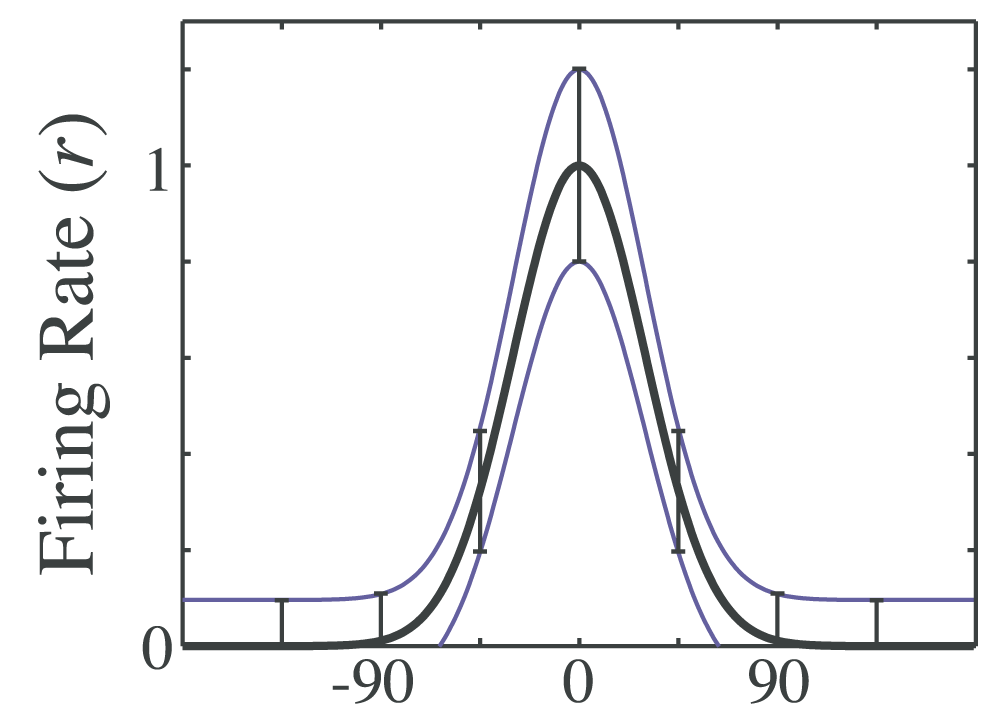
\includegraphics{figures/tuningcurve}
    \end{captionbeside}
\end{figure}

Given a population of neurons, also called a neural \emph{ensemble} in NEF terms, how can the encoded vector $\vc x(t)$ be recovered?
First the activity or spike trains $\act_i(t)$ are convolved with a synaptic filter $\syn$ to obtain the induced post-synaptic voltage change.
Usually this is a decaying exponential $\syn(t) = \syntau^{-1}\exp(-t / \syntau)$, but other filters can be used to more precisely model the dynamics of the synapse \parencite{voelker2017a} and even extensions to conductance-based synapses are possible \parencite{stockel2017}.
From the filtered activity, the represented vector can be reconstructed with a linear, weighted decoding
\begin{equation}
    \hat{\vc x}(t) = \sum_i \dec_i \cdot \sbr{a_i * h}\!(t)
\end{equation}
with decoding weights $\dec_i$.

To get a good reconstruction of the represented value, the decoding weights should minimize the error
\begin{equation}
    E = \int_{\repspace} \norm{\vc x - \hat{\vc x}}^2 \dif \vc x \text{.}
\end{equation}
In general, this minimization cannot be solved analytically.
Thus, in the NEF the integral is approximated by randomly sampling $M$ \emph{evaluation points} $\evalp_k \in \repspace$.
Given the finite number of evaluation points, it becomes possible to solve for the decoding weights with a least-squares minimization.
The detailed derivation is given in \textcite[Ch.~2]{eliasmith2003}.
In short, one obtains the matrices
\begin{equation}
    \actmat = \sbr{\begin{array}{cccc}
            \act_1(\vc x_1) & \act_1(\vc x_2) & \cdots & \act_1(\vc x_M) \\
            \act_2(\vc x_1) & \act_2(\vc x_2) & \cdots & \act_2(\vc x_M) \\
            \vdots & \vdots & \ddots & \vdots \\
            \act_N(\vc x_1) & \act_N(\vc x_2) & \cdots & \act_N(\vc x_M) \\
    \end{array}}
    \ \text{and}\ 
    \evalpmat = \sbr{\begin{array}{c}
            \vc x_1 \\ \vc x_2 \\ \vdots \\ \vc x_M
    \end{array}}
\end{equation}
where one can use the steady-state activities in the activity matrix $\actmat$ which can be obtained analytically for LIF neurons.
Given these two matrices the decoding weights can be obtained with the regularized pseudo-inverse as
\begin{equation}
    \sbr{\begin{array}{c}
            \dec_1\Tr \\ \dec_2\Tr \\ \vdots \\ \dec_N\Tr
        \end{array}} = \del{\actmat \actmat\Tr + M \reg^2 {\max(\actmat)}^2 \imat}^{-1} \actmat \evalpmat
\end{equation}
where $\reg$ is the regularization scale (usually $\reg = 0.1$).

The encoders and decoders not only allow us to encode information into a neural ensembles and decode it back out, but also to transmit that information from one neural population to another.
By decoding from the pre-synaptic ensemble and encoding into the post-synaptic ensemble, the connection weights required between the two populations can be obtained as
\begin{equation}
    \weights_{ij} = \enc_i\Tr \mat T \dec_j
\end{equation}
where $\mat T$ can describe a linear transform to implement across the neural connections.
If $\mat T$ is the identity matrix, the connection will be a pure communication channel.


\section{Transformation}
To be useful, a neural network has to transform or compute functions on the represented information.
In the NEF, it is straight-forward to implement a given transformation in the connection weights between two ensembles.
To implement a function $f(\vc x)$, one replaces the matrix $\evalpmat$ with
\begin{equation}
    \evalpmat_{f(\vc x)} = \sbr{\begin{array}{c}
            f(\vc x_1) \\ f(\vc x_2) \\ \vdots \\ f(\vc x_M)
    \end{array}}
\end{equation}
when solving for decoders.
This corresponds to a minimization of the modified error $E_{f(\vc x)} = \int_{\repspace} \norm{f(\vc x) - \hat{\vc x}}^2 \dif \vc x$.

\Textcite[Ch.~7]{eliasmith2003} shows that a neural network constructed in this way is typically best at computing low-order polynomials.
Non-smooth or discontinuous functions might require a large number of neurons.
In some cases a better function approximation can be achieved by appropriately selecting parameters like intercepts or encoders or by changing the network structure to decompose a function in a different way.
An example is the calculation of products and has been discussed in \textcite{gosmann2015-1}, and \cref{sec:thresholding} shows this for the thresholding of values.

\section{Dynamics}
The final principle of the NEF addresses dynamics.
In linear control theory a dynamical system is often described by state equations of the form
\begin{align}
    \od{\vc x}{t} &= \mat A \vc x(t) + \mat B \vc u(t) \label{eqn:statespace1} \\
    \vc y(t) &= \mat C \vc x(t) + \mat D \vc u(t) \label{eqn:statespace2}
\end{align}
where $\vc x(t)$ is the state vector, $\vc u(t)$ the input vector, and $\vc y(t)$ the output vector.
The system behaviour is determined by the dynamics matrix $\mat A$, input matrix $\mat B$, output matrix $\mat C$, and the feedthrough matrix $\mat D$.
\Cref{fig:statespace} shows a graphical representation.
\begin{figure}
    \centering
    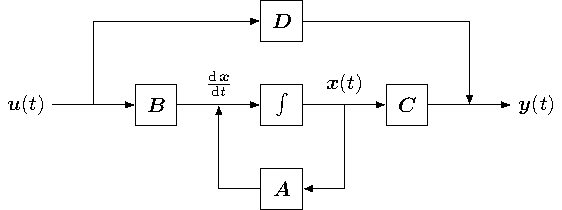
\includegraphics{tikz/statespace}
    \caption{Visualization of \cref{eqn:statespace1,eqn:statespace2} as block diagram.}\label{fig:statespace}
\end{figure}

In the NEF, we want to map a given dynamical system onto neural components (\cref{fig:neural-lti}).
The neuron dynamics are dominated by the synaptic filter \parencite[Appendix~F.1]{eliasmith2003} which becomes the transfer function and gives
\begin{equation}
    \vc x(t) = \syn(t) * \sbr{\mat A' \vc x(t) + \mat B' \vc u(t)} \text{.}
\end{equation}
With help of the Laplace transform one can obtain $\mat A'$ and $\mat B'$ from $\mat A$ and $\mat B$ as
\begin{align}
    \mat A' &= \syntau \mat A + \imat \\
    \mat B' &= \syntau \mat B  \text{.}
\end{align}
This implies that to implement a dynamical system with a neural ensemble, the input has to be multiplied by $\syntau$ to account for the synaptic filtering.
In addition, one needs to add a recurrent transformation implementing the function $f(\vc x) = \syntau \mat A \vc x + \vc x$.
Note that combining this third principle with the principle of transfomation, allows the implementation of nonlinear dynamics in a spiking neural network.
\begin{figure}
    \centering
    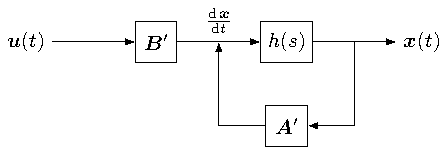
\includegraphics{tikz/neural-lti}
    \caption[Block diagram of the linear system of a neural population.]{Block diagram of the linear system of a neural population. $h(s)$ is the Laplace transformed synaptic filter $\syn(t)$.}\label{fig:neural-lti}
\end{figure}


\section{Simulating NEF networks}
To simulate NEF style networks, I use the Python library Nengo \parencite{bekolay2014,sharma2016}.
It supports different backends to run neural models on different hardware platforms.
For example, Nengo OCL targets GPUs with an OpenCL implementation.
While this allows better simulation performance, special case implementations are necessary for certain features.
In particular, this applies to the association matrix learning rule (see \cref{sec:aml}).
Moreover, I utilized the Sharcnet and Compute Canada high-performance clusters which typically provide more CPU resources than GPU resources.
Thus, I mostly used the Nengo reference (CPU) backend.
To obtain sufficient simulation performance for the size of models constructed in this work, it was necessary to optimize memory organization of the internal data structures of the backend.
While the exact details are out of the scope of this thesis, they are published in \textcite{gosmann2017}.

\chapter{The Semantic Pointer Architecture}\label{sec:spa}
While the Neural Engineering Framework allows us to encode vectors into spiking neural networks and transform them, it does not tell us how to use those vectors to represent structured, conceptual, or symbol-like information.
Different such methods could be devised, though in the context of the NEF the most widely used method is the Semantic Pointer Architecture \parencite[SPA;][]{eliasmith2013}.
The SPA has been used to build a multitude of cognitive models, including the n-back task \parencite{gosmann2015}, the Tower of Hanoi task \parencite{stewart2011-2}, human-scale knowledge representation \parencite{crawford2016}.
The largest and most complex example of a SPA model is Spaun, the Semantic Pointer Architecture Unified Network, combining eight different tasks in a single functional spiking-neuron model \parencite{Eliasmith2012}.

The conceptual representations in the SPA are a specific instance of a Vector Symbolic Architecture \parencite[VSA;][]{gayler2004}.
In VSAs concepts are represented with vectors, and linear and nonlinear operators are used to combine basic concepts in more complex structured representations.
Three types of operators are considered essential in a VSA\@.
First, a measure of similarity
\begin{equation}
    \simmeasure: \mathbb{R}^{\dims} \times \mathbb{R}^{\dims} \longrightarrow \mathbb{R}
\end{equation}
for which I use the normalized dot product (also known as cosine similarity)
\begin{equation}
    \simmeasure(\vc x, \vc y) := \frac{\left\langle \vc x, \vc y \right\rangle}{\norm{\vc x} \cdot \norm{\vc y}}
\end{equation}
for the remainder of this thesis.
Second, a superposition operator
\begin{equation}
    \superpos: \mathbb{R}^{\dims} \times \mathbb{R}^{\dims} \longrightarrow \mathbb{R}^{\dims}
\end{equation}
is required that produces a vector similar to both inputs, i.e., $\simmeasure(\superpos(\vc x, \vc y), \vc x) \approx \simmeasure(\superpos(\vc x, \vc y), \vc y) \gtrapprox \sqrt{1/2}$ for $\simmeasure(\vc x, \vc y) \approx 0$.
This is usually, and will be for the remainder of this thesis, simple elementwise addition, i.e., $\superpos(\vc x, \vc y) := \vc x + \vc y$.
Finally, a binding operator
\begin{equation}
    \bind: \mathbb{R}^{\dims_1} \times \mathbb{R}^{\dims_2} \longrightarrow \mathbb{R}^{\dims}
\end{equation}
is needed with an approximate inverse or unbinding operation
\begin{equation}
    \bind^+: \mathbb{R}^d \times \mathbb{R}^{\dims_2} \longrightarrow \mathbb{R}^{\dims_1} \text{.}
\end{equation}
To be able to build up and retrieve information from representations, the binding and unbinding operations are required to be distributive, i.e.,
\begin{align}
    \bind(\vc x + \vc y, \vc z) &= \bind(\vc x, \vc z) + \bind(\vc y, \vc z) \\
    \bind^+(\vc x + \vc y, \vc z) &= \bind^+(\vc x, \vc z) + \bind^+(\vc y, \vc z) \text{.}
\end{align}

For some proposed binding operations, like Tensor products \parencite{smolensky1990}, the unbinding operation is the exact inverse $\bind^+ = \bind^{-1}$ with
\begin{equation*}
    \bind^{-1}(\bind(\vc x, \vc y), \vc y) = \vc x \text{.}
\end{equation*}
However, Tensor products increase the vector dimensionality with each successive binding which leads to biological implausible scaling problems \parencite[Appendix D.5]{eliasmith2013}.
For that reason, I only consider binding methods that keep the dimensionality $\dims = \dims_1 = \dims_2$ constant.

In pure math, it is still possible to define binding operators with an exact inverse, but we need to keep the implementation in neurons in mind.
This introduces additional constraints.
First, the actual usable representational space $\repspace \subsetneq \mathbb{R}^{\dims}$ is limited, constraining unlimited growth of bound vectors.
Second, neural noise limits the representational accuracy, preventing highly non-linear operators.
It follows that for a binding operator in a neural system it is desired to maximize the set $\mathcal{V} \subseteq \repspace$ for which  $\simmeasure(\bind^+(\bind(\vc x, \vc y) + \vc\zeta, \vc y), \vc x) \approx 1$ for all $\vc x, \vc y \in \mathcal{V}$ and samples of noise $\vc\zeta$ in the neural system.
Note that this condition would be satisfied by using the identity $\bind(\vc x, \vc y) = \bind^+(\vc x, \vc y) = \vc x$.
Thus, simultaneously it needs to hold that $\simmeasure(\bind^+(\bind(\vc x, \vc y), \vc z), \vc x) \approx 0$ for all $\vc x, \vc y, \vc z \in \mathcal{V}$ with $\simmeasure(\vc y, \vc z) \approx 0$.
At this point, it is useful to introduce three more definitions.

\begin{defn}[identity vector]
    A vector $\bid_{\bind}$ with the property $\bind(\vc x, \bid_{\bind}) = \vc x$ is called \emph{identity vector} under $\bind$.
\end{defn}
\begin{defn}[absorbing element]
    A vector $\bzero_{\bind}$ with the property $\bind(\vc x, \bzero_{\bind}) = c \cdot \bzero_{\bind}$ where $c \in \mathbb{R}$ is called an \emph{absorbing element} under $\bind$.
\end{defn}
Such an absorbing element effectively destroys the information in the vector $\vc x$.
For that reason, absorbing elements should be avoided when constructing representations with binding.
Note that this definition slightly differs from the usual definition of absorbing elements by allowing for a scaling factor.
\begin{defn}[unitary vector]
    A vector $\vc u$ with the property $\langle \bind(\vc x, \vc u), \bind(\vc y, \vc u) \rangle = \langle \vc x, \vc y \rangle$ is called unitary.
\end{defn}
In other words, a unitary vector preserves the dot product under binding.
This is in analogy to unitary transformation matrices that also preserve the dot product.
It also implies that binding with a unitary vector preserves the length of the bound vector.


\section{Binding operations}
I introduce two specific binding operations now.
First, circular convolution is discussed, which has been the binding operation of choice in the SPA so far.
Second, I introduce a new binding method, termed vector-derived transformation binding, with some trade-offs.
The two binding approaches and their suitability for different problems is discussed.

\subsection{Circular convolution}
The binding operator classically used in the SPA is circular convolution, and was suggested by \textcite{plate1995,plate2003} for his Holographic Reduced Representations (HRRs).
\begin{defn}[circular convolution binding]
    The circular convolution binding operator is given by
    \begin{equation}
        \bind_{\circledast}(\vc x, \vc y) := \vc x \circledast \vc y\ \text{with}\ \del{\vc x \circledast \vc y}_i = \sum_{j=0}^{d - 1} x_j y_{(i - j) \bmod d}
    \end{equation}
    and has the approximate inverse \parencite{plate2003}
    \begin{equation}
        \bind^+_{\circledast}(\vc x, \vc y) = \vc x \circledast \vc y^+\ \text{with}\ \vc y^+ := \del{y_0, y_{d-1}, y_{d-2}, \dotsc, y_1}\Tr \text{.}
    \end{equation}
\end{defn}

The basic properties of
\begin{align}
    &\text{distributivity:} &(\vc x_1 + \vc x_2) \circledast \vc y &= \vc x_1 \circledast \vc y + \vc x_2 \circledast \vc y \text{,}\\
    &\text{associativity:} &(\vc x \circledast \vc y) \circledast \vc z &= \vc x \circledast (\vc y \circledast \vc z) \text{,} \\
    &\text{commutativity:} &\vc x \circledast \vc y &= \vc y \circledast \vc x
\end{align}
hold for circular convolution as a binding operator.
A useful property of circular convolution for the implementation in a neural network with the NEF is, that it becomes element-wise multiplication in the Fourier space defined by
\begin{equation}
    \vc x \circledast \vc y = \fouriermat^{-1}\sbr{(\fouriermat \vc x) \circ (\fouriermat \vc y)}
\end{equation}
where $\fouriermat$ is the discrete Fourier transform (DFT) matrix.
The linear transform with the DFT matrix can be put easily into the neural connection weights and the element-wise product can be done with a well-optimized product network \parencite{gosmann2015-1}.

The expression in Fourier space also allows the derivation of the special elements of circular convolution.
The identity vector must not change the complex Fourier coefficient in the element-wise multiplication.
Thus, its Fourier coefficients must all be $1 + 0\iu$ and the identity vector is given by
\begin{equation}
    \bid_{\circledast} = (1, 0, 0, \dotsc, 0)\Tr \text{.}
\end{equation}
Furthermore, all vectors with Fourier coefficients $c_n \in \mathbb{C}$ that have an absolute value of $\left|c_n\right| = 1$ are unitary, as one can easily verify.
A trivial example of a unitary vector is the identity vector $\bid_{\circledast}$.
Finally, all vectors $(z, \dotsc, z)\!\Tr$ with $z \in \mathbb{R}$ are absorbing elements.

\subsection{Vector-derived transformation binding}
Circular convolution can be interpreted as moving one of the operands around in the $d$-dimensional space in a way defined by the other operand.
This leads to the question, whether there are other ways to project one vector to a new location based on the other vector.
One such way is what I call \emph{vector-derived transformation binding (VTB)}, which to my knowledge has not been described before.
\begin{defn}[vector-derived transformation binding, VTB]
    Given a $\dims' = \dims^{\frac{1}{2}} \in \posnum$, the vector-derived transformation binding operator $\vtb: \mathbb{R}^{\dims} \times \mathbb{R}^{\dims} \longrightarrow \mathbb{R}^{\dims}$ is defined as
    \begin{equation}
        \vtb(\vc x, \vc y) := \bar{\mat V}_{\vc y} \vc x = \begin{bmatrix}
            \mat V_{\vc y} & 0 & 0 \\
            0 & \mat V_{\vc y} & 0 \\
            0 & 0 & \ddots
        \end{bmatrix} \vc x
    \end{equation}
    with
    \begin{equation}
        \mat V_{\vc y} = \dims^{\frac{1}{4}} \begin{bmatrix}
            y_1 & y_2 & \dotso & y_{\dims'} \\
            y_{\dims' + 1} & y_{\dims' + 2} & \dotso & y_{2\dims'} \\
            \vdots & \vdots & \ddots & \vdots \\
            y_{\dims - \dims' + 1} & y_{d - \dims' + 2} & \dotso & y_{\dims}
        \end{bmatrix} \text{.}
    \end{equation}
    The approximate inverse is given by
    \begin{equation}
        \vtb^+(\vc x, \vc y) = \bar{\mat V}_{\vc y}\Tr \vc x = \begin{bmatrix}
            V_{\vc y}\Tr & 0 & 0 \\
            0 & V_{\vc y}\Tr & 0 \\
            0 & 0 & \ddots
        \end{bmatrix} \vc x \text{.}
    \end{equation}
\end{defn}
This binding method is based on the fact that in the SPA vectors are usually randomly generated and uniformly distributed with identically distributed components.
In that case each subvector (e.g., each row in $\mat V_{\vc y}$) is also uniformly distributed with identically distributed components.
Furthermore, for high-dimensional vector spaces almost all (uniformly sampled) vectors are orthogonal and semantic pointers are usually picked to have unit-length.
Thus, the matrix $\bar{\mat V}_{\vc y}$ is almost orthogonal with the implication $\bar{\mat V}_{\vc y}\Tr \bar{\mat V}_{\vc y} \approx \imat$.
Vectors $\vc y$ that give a perfectly orthogonal matrix $\mat V_{\vc y}$, are unitary.
One special unitary vector is the identity vector.
\begin{corollary}[VTB identity vector]
    The identity vector for VTB is given by
    \begin{equation}
        \sbr{\bid_{\ped{V}}}_i = \left\{ \begin{array}{ll}
                \dims^{-\frac{1}{4}} & i \in \cbr{(k - 1) \dims' + k : k \leq \dims', k \in \mathbb{N}_{>0}} \\
                0 & \text{otherwise}
        \end{array}\right. \text{.}
    \end{equation}
    \begin{proof}
        By writing $\bid_{\ped{V}}$ as $\mat V_{\bid_{\ped{V}}}$ one can easily verify that $\mat V_{\bid_{\ped{V}}} = \imat\ \Rightarrow\ \bar{\mat V}_{\bid_{\ped{V}}} = \imat$.
    \end{proof}
\end{corollary}
Example for $d = 9$: $\bid_{\ped{V}}^{(9)} = (1, 0, 0, 0, 1, 0, 0, 0, 1)\Tr$.

\begin{corollary}[VTB distributivity]
    VTB is distributive:
    \begin{equation}
        \begin{split}
            \vtb(\vc x_1 + \vc x_2, \vc y) &= \vtb(\vc x_1, \vc y) + \vtb(\vc x_2, \vc y) \text{ and}\\
            \vtb(\vc x, \vc y_1 + \vc y_2) &= \vtb(\vc x, \vc y_1) + \vtb(\vc x, \vc y_2) \text{.}
        \end{split}
    \end{equation}
    \begin{proof}
        By applying the definitions for both directions of the distributivity:
        \begin{itemize}
            \item $\vtb(\vc x_1 + \vc x_2, \vc y) = \bar{\mat V}_{\vc y} \del{\vc x_1 + \vc x_2} = \bar{\mat V}_{\vc y} \vc x_1 + \bar{\mat V}_{\vc y} \vc x_2 = \vtb(\vc x_1, \vc y) + \vtb(\vc x_2, \vc y)$
            \item $\vtb(\vc x, \vc y_1 + \vc y_1) = \bar{\mat V}_{\vc y_1 + \vc y_2} \vc x = \del{\bar{\mat V}_{\vc y_1} + \bar{\mat V}_{\vc y_2}} \vc x = \bar{\mat V}_{\vc y_1} \vc x + \bar{\mat V}_{\vc y_2} \vc x = \vtb(\vc x, \vc y_1) + \vtb(\vc x, \vc y_2)$
    \end{itemize}
    \end{proof}
\end{corollary}
In contrast to circular convolution, VTB is neither commutative
\begin{equation}
    \vtb(\vc x, \vc y) = \bar{\mat V}_{\vc y} \vc x \neq \bar{\mat V}_{\vc x} \vc y = \vtb(\vc y, \vc x) \text{,}
\end{equation}
nor associative
\begin{equation}
    \vtb(\vc x, \vtb(\vc y, \vc z)) = \bar{\mat V}_{\bar{\mat V}_{\vc z} \vc y} \vc x \neq \bar{\mat V}_{\vc z} \bar{\mat V}_{\vc y} \vc x = \vtb(\vtb(\vc x, \vc y), \vc z) \text{.}
\end{equation}
This implies that unlike circular convolution, multiple bindings cannot be undone in a single step, but a separate unbinding step is required for each binding.
Despite the non-commutativity, it is possible to flip the operands in the bound state $\vtb(\vc x, \vc y) = \mat V_{\leftrightarrow} \vtb(\vc y, \vc x)$ with the matrix
\begin{equation}
    \sbr{\mat V_{\leftrightarrow}}_{ij} = \left\{ \begin{array}{ll}
            1 & j = 1 + \left\lfloor \frac{i - 1}{\dims'} \right\rfloor + \dims' \sbr{\del{i - 1} \bmod \dims'} \\
            0 & \text{otherwise}
        \end{array}\right. \text{.}
\end{equation}
Example for $d = 4$:
\begin{equation*}
    \mat V_{\leftrightarrow}^{(4)} = \sbr{\begin{array}{cccc}
            1 & 0 & 0 & 0 \\
            0 & 0 & 1 & 0 \\
            0 & 1 & 0 & 0 \\
            0 & 0 & 0 & 1
        \end{array}}
\end{equation*}

\subsection{Comparison of circular convolution and vector-derived transformation binding}
Both circular convolution and VTB are compressed binding operations.
Because of the lossy compression, we lose some information in each binding which makes it increasingly harder to recover the original unbound vectors.
To combat this effect (and the effect of neuron noise) clean-up memories like the one by \textcite{stewart2011} are required.
Likewise the independent accumulator model discussed in \cref{sec:ia} can be used as a clean-up memory.

In addition to the information loss, the binding operations change the length of the vector (if neither operand is unitary).
This can be a problem in a neural representation as neurons saturate and might not represent the vector accurately anymore.
In particular, neural ensembles in the NEF are optimized for a certain representational space, usually a hyperball with a given radius $\radius$.
It is convenient to set $\radius = 1$ and try to keep the Semantic Pointer vectors at unit-length.

\Cref{fig:bindings-autoconv} shows how the mean length of random vectors repeatedly bound with themselves changes.
For the circular convolution the length increases much faster than for VTB\@.
Such a rapid increase in length can be problematic in a neural network with a limited representational radius as in the NEF\@.
Moreover, VTB preserves more information of the bound vectors as shown by the similarity to the original vectors when undoing all bindings.
After repeated binding with itself and then the same number of unbindings, the resulting VTB bound vector is more similar to the original vector than the circular convolution bound vector.
\begin{figure}
    \centering
    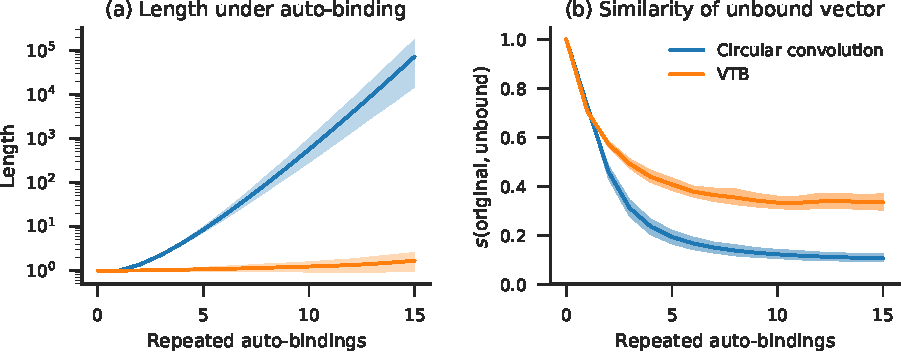
\includegraphics{figures/bindings-autoconv}
    \caption[Repeatedly binding a 256-dimensional vector with itself.]{Repeatedly binding a 256-dimensional vector with itself. (a) Length of the resulting vector. (b) Similarity of the original vector to the vector obtained when undoing all bindings. The shaded areas represent \SI{95}{\percent} confidence intervals.}\label{fig:bindings-autoconv}
\end{figure}

While binding vectors with themselves can sometimes be useful (e.g., for generating Semantic Pointers with a successive relationship like position indices), it is much more common to bind randomly sampled vectors.
\Cref{fig:bindings-random} shows the same experiment where a random vector was used in each binding.
In this case, the vector length decreases to zero, even if it might increase in some of the early bindings.
Again, this decrease is much quicker for circular convolution binding than for VTB and the latter method also preserves more of the similarity across bindings.
\begin{figure}
    \centering
    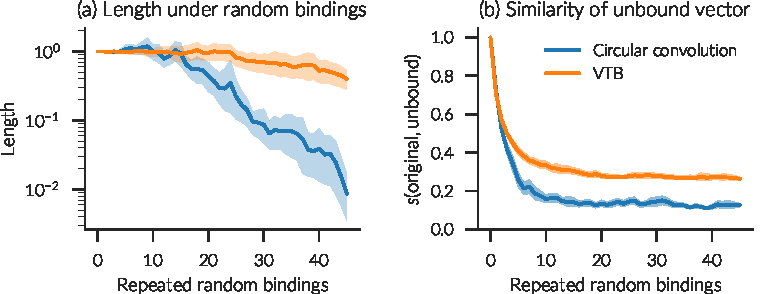
\includegraphics{figures/bindings-random}
    \caption[Repeatedly binding a 256-dimensional vector with random vectors.]{Repeatedly binding a 256-dimensional vector with random vectors. (a) Length of the resulting vector. (b) Similarity of the original vector to the vector obtained when undoing all bindings. The shaded areas represent \SI{95}{\percent} confidence intervals.}\label{fig:bindings-random}
\end{figure}

It is conceivable that the problems with scaling of the vector length can be fixed by normalizing after each binding.
This, however, does not affect the loss of information in each binding (\cref{fig:bindings-normalized}).
Also, implementing normalization in a neural network is notoriously difficult because of the division involved with an unbounded output as the divisor approaches zero.
Good approximations of normalization are only possible for a defined and finite input range.
It is worth noting that the neurons in the NEF perform a sort of ``soft normalization'' for large values, as the neuron's firing rates saturate.
But this only affects vectors exceeding a certain length and can lead to other distortions in the representation.
\begin{figure}
    \centering
    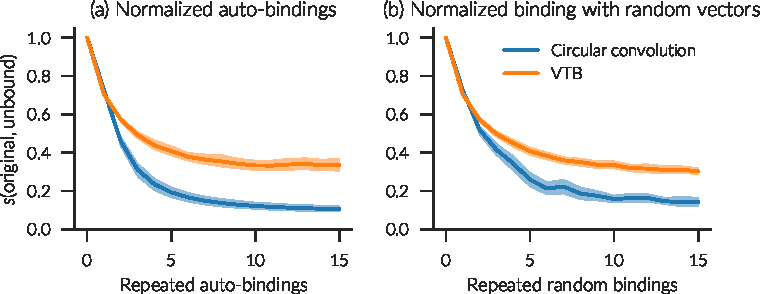
\includegraphics{figures/bindings-normalized}
    \caption[Repeatedly binding a 256-dimensional vector with normalization.]{Repeatedly binding a 256-dimensional vector with (a) itself or (b) random vectors and normalizing in each step. The similarity to the original vector after undoing all bindings is shown. The shaded areas represent \SI{95}{\percent} confidence intervals.}\label{fig:bindings-normalized}
\end{figure}

Another approach to preventing the growth or decay of the vector length, and even prevent the information loss, is the usage of unitary vectors.
These keep the vector length constant and perform lossless binding due to their perfect inverse.
Note that binding two unitary vectors gives another unitary vector.
Thus, repeated binding is not a problem.
However, the scaling properties of VSAs are based on the fact that the number of almost orthogonal vectors that fits into a vector space grows exponentially with the dimensionality of that space \parencite{wyner1967,cai2013}.
Because not all vectors are unitary, this scaling property might be lost when restricted to unitary vectors.
It might be best to use unitary vectors only for those Semantic Pointers that are repeatedly used in bindings.
But it is also worth keeping in mind that achieving the theoretical limit of almost orthogonal vectors in a space is a hard problem, closely related to sphere packing and unsolved for arbitrary dimensionality \parencite{cohn2017}.
Thus, the practical scaling of the number of useable vectors might be less then the exponential scaling for both unitary and non-unitary vectors.

So far VTB looks like the better choice for a binding operation.
But it does not come not without downsides.
In contrast to circular convolution, it is not associative or commutative.
While the desirability of commutativity depends on the employed representation scheme, the non-associativity implies that each binding has to be undone in an individual step, while circular convolution allows us to undo a chain of bindings in a single step, if the vector representing that chain is available.
Thus, circular convolution can allows the recovery of information more quickly.
Ultimately, this is a question of what binding operations the brain applies for different forms of processing (if such binding is at all related to what the brain does).
Potentially, the binding operations lead to different timing predictions, as unbinding with the VTB may take more time.
Deriving such predictions and testing them experimentally is, however, out of the scope of this thesis.

Finally, we have to consider the neural implementation of these binding operations.
Both essentially require a set of multiplication networks.
For the circular convolution, the DFT (and inverse DFT) can be implemented in feed-forward connection weights that do not require any additional neurons.
For each of the input vectors $\dims$ Fourier complex coefficients are produced, but as the inputs are real-valued, half of these are the complex conjugate of the other half.
Thus, only $\dims / 2$ coefficients have to be considered.
Each coefficient is a complex number multiplied with one coefficient of the other vector.
That results in four real-valued multiplies per coefficient.
In total, $2\dims$ multiplications are required for a circular convolution.
For VTB, there are $\dims^{1/2}$ multiplications of $\dims^{1/2} \times \dims^{1/2}$ matrices with a vector, resulting in a total of $\dims^{3/2}$ multiplications.
However, each column vector in $\bar{\mat V}_{\vc y}$ gets scaled by the same component of $\vc x$.
That would allow, to store each of these column vectors in a single NEF ensemble with the respective $x_i$ in an additional dimension, and then decode the scaled column vector.
This requires only $\dims$ ensembles to decode from, but each ensemble needs to represent $\dims^{1/2} + 1$ dimensions, and to keep the noise error constant (as discussed in the next chapter), the number of neurons in each ensemble then needs to be scaled by ${(\dims^{1/2} + 1)}^{3/2} \approx \dims^{3/4}$.
Overall ensembles this amounts to a scaling by $\dims^{7/4}$.
Thus, the VTB requires more neural resources.
It should be noted, that for either binding method, the binding with a fixed vector can be implemented purely in the connection weights as it reduces to a simple matrix multiplication in either case.

Despite VTB having many advantages over circular convolution, I decided to use circular convolution in the memory model.
The main reason is that support for circular convolution is already implemented in Nengo and the model does not use a lot of binding operations.
Nevertheless, it would be interesting to switch the model over to VTB and investigate effects on the performance in the future.


\section{Structured representations}
Once we defined a binding operation, it can be used to build up structured representations with Semantic Pointers.
For example, consider a scene with a red square and blue circle that we want to encode as Semantic Pointer.
Assume that we have Semantic Pointers \spc{red}, \spc{square}, \spc{blue}, and \spc{circle}.
One possible encoding would be
\begin{equation}
    \vc s = \bind(\spc{red}, \spc{square}) + \bind(\spc{blue}, \spc{circle}) \text{.}
\end{equation}
We could then recover the color of the square as
\begin{align}
    \bind^+(\vc s, \spc{color}) &= \bind^+(\bind(\spc{red}, \spc{square}), \spc{square}) + \bind^+(\bind(\spc{blue}, \spc{circle}), \spc{square}) \\
    &\approx \spc{red} + \mathrm{noise} \text{.}
\end{align}
Note, however, that the binding operation needs to be commutative to recover the shape from the color with this encoding scheme.
Other encoding schemes can be devised to alleviate this concern.
For example, the properties can be bound to a role and each object to an object identifier:
\begin{align}
    \vc o_1 &= \bind(\spc{red}, \spc{color}) + \bind(\spc{square}, \spc{shape}) \\
    \vc o_2 &= \bind(\spc{blue}, \spc{color}) + \bind(\spc{circle}, \spc{shape}) \\
    \vc s &= \bind(\vc o_1, \spc{obj}_1) + \bind(\vc o_2, \spc{obj}_2) \text{.}
\end{align}
To find the color of a specific shape, each object would have to be retrieved, then the shape of the object to compare it to the target shape, and finally the color has to recovered if the shape matches.
Thus, different encoding schemes can lead to different timing predictions.
The latter approach requires scanning and through multiple objects and thus it should take longer to recover information with more items, while the former approach can recover any property in a single step.
Despite those differences, both encoding approaches are similar, in so far as pairs of semantic pointers are bound together.
\begin{defn}[encoding with binding]
    Given $k$ pairs $(\vc x_i, \vc y_i) \in \mathbb{R}^{\dims} \times \mathbb{R}^{\dims}$, the encoding of these pairs into a single Semantic Pointer $\vc m$ with binding is given by
    \begin{equation}
        \vc m = \sum_{i=1}^k \bind(\vc x_i, \vc y_i) \text{.}
    \end{equation}
\end{defn}
An $\vc x_i$ from such a trace can be recalled as $\vc x_i \approx \hat{\vc x}_i = \bind^+(\vc m, \vc x_i)$.
While most concrete encoding schemes make use of encoding with binding, at least one other method, encoding with tagging, has been proposed \parencite{recchia2015}.
\begin{defn}[encoding with tagging]
    Given $k$ pairs $(\vc x_i, \vc y_i) \in \mathbb{R}^{\dims} \times \mathbb{R}^{\dims}$ and a matrix $\mat M \in \mathbb{R}^{\dims \times \dims}$ with an approximate inverse $\mat M^+$ satisfying $\mat M^+ \mat M \approx \imat$, the encoding into a single Semantic Pointer with tagging is given by
    \begin{equation}
        \vc m = \sum_{i=1}^k \mat M^{2i-1} \del{\vc y_i + \mat M \vc x_i} = \sum_{i=1}^k \mat M^{2i-1} \vc y_i + \mat M^{2i} \vc x_i \text{.}
    \end{equation}
\end{defn}
The retrieval of an $\vc x_i \approx \hat{\vc x}_i$ is accomplished with
\begin{align}
    \hat{\vc x}_i &:= \del{\mat M^{2c}}^+ \vc m \\
    c &= \argmax_{j \in \sbr{1, k}}\ \simmeasure\!\del{\vc y_i, \del{\mat M^{2j-1}}^{\!+} \vc m} \text{.}
\end{align}

There are a number of sensible choices for the matrix $\mat M$.
\begin{itemize}
    \item First of all, for both, circular convolution and VTB, binding with a \emph{fixed} vector $\vc v$ can be expressed as a matrix multiplication.
        A matrix $\mat M$ derived in this way is unitary, if and only if the vector $\vc v$ is unitary for the given binding operation.
    \item A common choice for encoding with tagging are permutation matrices.
        These are unitary and an exact inverse is given by the transpose.
    \item A special permutation matrix is the matrix that shifts all vector components by one.
        For a given permutation matrix, the vector space dimensions can be reordered such that the permutation matrix becomes the shift by one.
        Interestingly, the shift by one is also equivalent to a circular convolution with the vector $(0, 1, 0, 0, \dotsc)\Tr$.
    \item Other good candidates for $M$, that have not been considered to my knowledge, are (random) orthogonal matrices.
        These are unitary operators on $\mathbb{R}^{\dims}$ and thus have an exact inverse given by the transpose.
\end{itemize}
The relations of these different matrix choices is shown in the Venn diagram in \cref{fig:tagging-matrices}.
\begin{figure}
    \centering
    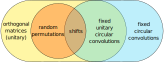
\includegraphics[scale=0.85]{figures/tagging-matrices}
    \caption[Venn diagram of matrices for encoding with tagging.]{Venn diagram of the relations between different classes of matrices $\mat M$ that can be used for encoding with tagging.}\label{fig:tagging-matrices}
\end{figure}

Either encoding method allows the recovery of encoded vectors, but the encoding vector itself is (in general) not similar to those encoded vectors.
In this way, the vector is analogous to a pointer in computer science that doesn't directly contain the information, but can be dereferenced to access the information it is pointing to.
Unlike pointers, however, these vectors can also capture semantic information by their distance in vector space.
Due to the combination of these two facts, these vectors are called Semantic Pointers. 


\subsection{Comparison of encoding methods}
Based on experiment~1 from \textcite{recchia2015}, the encoding methods can be compared by measuring the pairwise binding capacity.
To do so, a set of \num{1000}~vectors with normally distributed components $x_i \sim \ndist\!\del{\!0, \sqrt{1/\dims}}$ are created (note that $\expected\!\sbr{\,\norm{\vc x}} = 1$).
From this set \num{500}~pairs are sampled with replacement.
Then $k$ of these pairs are encoded into a single vector and it is tested whether the $\vc x$ of a random encoded pair $(\vc x, \vc y)$ can recovered with the cue $\vc y$.
A vector counts a successfully recovered if $\hat{\vc x}$ is more similar to $\vc x$ than any other vector in the initial set of vectors.
\num{1000} trials were run and averaged over for each encoding scheme and vector dimensionality.
Because VTB requires the dimensionality~$\dims$ to be square, \num{256}, \num{484}, \num{1024}, and \num{2025} were picked.

\Cref{fig:encoding}a shows the results for encoding with binding.
Both binding operators perform about the same.
While this experiment essentially follows \textcite{recchia2015}, it gives much better results.
It is not clear whether they omitted an essential detail from their description or whether their implementation of the binding operation is flawed.
\begin{figure}
    \centering
    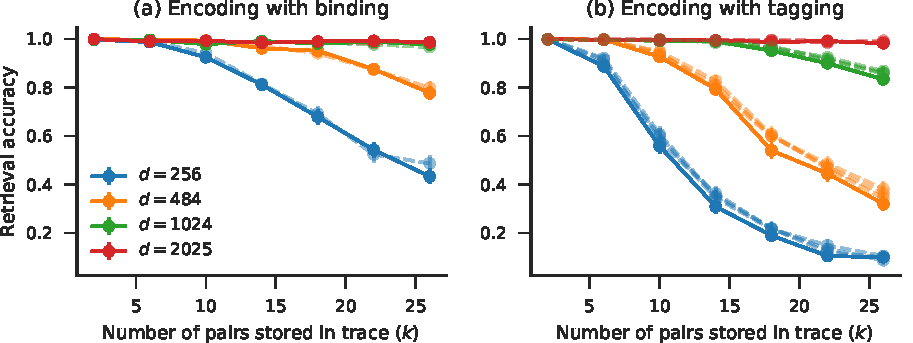
\includegraphics{figures/encoding}
    \caption[Retrieval accuracy of encoding methods.]{Retrieval accuracy for (a) encoding with binding and (b) encoding with unitary tagging matrices. Solid lines show results for VTB\@. The dashed lines in (a) show results for binding with circular convolution, in (b) results for unitary circular convolution matrices, shift matrices, and orthogonal matrices without further indication as the results are almost identical. Error bars denote \SI{95}{\percent} confidence intervals.}\label{fig:encoding}
\end{figure}

The results for encoding with tagging by a shift of one are shown in \cref{fig:encoding}b and closely match the results presented in \textcite{recchia2015}.
Note that the same result applies to any other permutation matrix as the vector components can be reordered accordingly.
Very similar results are obtained with orthogonal matrices, fixed unitary circular convolution, and unitary VTB\@.
In all these cases, the pairwise binding capacity is below the encoding with binding, opposed to what \textcite{recchia2015} reported.
Intuitively, this can be explained by the fact that encoding with binding is a sum of $k$ vectors, where each vector has encoded information about the pair's constituents, whereas encoding with tagging is a sum of $2k$ vectors because each pair's constituent gets encoded separately.
In other words, encoding with binding has a pairwise binding capacity about twice as high as encoding with tagging.
In the plots, the retrieval accuracies for encoding with binding at $2k$ matches roughly with the retrieval accuracy with tagging at $k$, illustrating this fact.

Finally, we can observe (\cref{fig:encoding-nonunitary-tagging}) that encoding with tagging completely fails with fixed non-unitary circular convolution matrices and does not do much better with non-unitary VTB matrices either.
This is likely due to the fact that repeated circular convolution with the same (non-unitary) vector leads to a super-exponential increase in length.
That causes one pair (or even one vector of that pair) to be much stronger than all the other pairs, preventing their recovery.
\begin{figure}
    \centering
    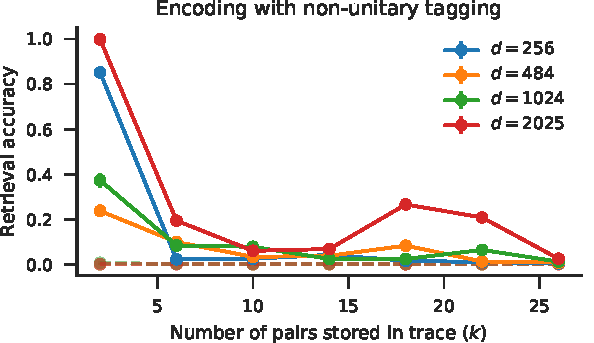
\includegraphics{figures/encoding-nonunitary-tagging}
    \caption[Retrieval accuracy of encoding with non-unitary tagging matrices.]{Retrieval accuracy for encoding with non-unitary tagging matrices. Solid lines show results for VTB matrics, while dashed lines show results for circular convolution matrices. Error bars for \SI{95}{\percent} confidence intervals are smaller than then marker size.}\label{fig:encoding-nonunitary-tagging}
\end{figure}

These experiments clearly show that encoding with binding is preferable.
Even more so, as retrieving items from an encoding with tagging is much more involved.
Each potential cue vector $\vc y_i$ has to be recovered and compared to the actual cue $\vc y$ to determine the maximum similarity to the cue, and which $\vc x_i$ has to be decoded from the encoding.
The encoding with binding allows direct querying of an $\vc x_i$ with a given $\vc y_i$.
This makes for a simpler implementation in a neural network.
That being said, if the main concern is not the implementation in a neural network, but the performance of the vector operations on a classical digital computer, one might come to a different conclusion as \textcite{recchia2015} did.

\chapter{Optimized high-dimensional representation in spiking neurons}
The implementation of a Semantic Pointer Architecture in a spiking neural network requires the representation of high-dimensional vectors.
While the standard NEF already provides us with a method to do this, it does not tell us the best way to do so.
A good representation will try to minimize the error or noise in the representation.
Alternatively, if the error is sufficiently small, it allows to reduce the number of neurons which reduces the simulation run time.
I previously proposed an optimization method for the representation~\parencite{gosmann216}, which improved the accuracy of SPA operations by up to 25 times.
Here, I will describe a more general applicable method that matches or exceeds the performance of the method among some other advantages.

\section{Types of error in neural representations}
In the NEF the total representational error is given by
\begin{equation}
    \errtotal^2 = \left\langle \errtotal^2(\vc x) \right\rangle_{\!\vc x \in \repspace} = \left\langle \norm{\vc x - \hat{\vc x}(t)}^2 \right\rangle_{\!t,\,\vc x \in \repspace} \text{.}
\end{equation}
As detailed by \textcite[47--48]{eliasmith2003} the total error is constituted out of the error caused by spiking noise $\errnoise$ and the error due to the static distortion $\errdist$ from the non-perfect decoding:
\begin{align}
    \errtotal^2(\vc x) &= \errnoise^2(\vc x) + \errdist^2(\vc x) \\
    \errnoise(\vc x) &= \left\langle \norm{\hat{\vc x}(t) - \langle \hat{\vc x}(t) \rangle_{\!t}}^2 \right\rangle_{\!t} \\
    \errdist(\vc x) &= \norm{\vc x - \langle \hat{\vc x}(t) \rangle_{\!t}}^2 \text{.}
\end{align}
The relation of the error terms is explained by the partitioning of the sum of squares in ordinary least squares model (which is used to solve for decoders in the NEF).
Note that the noise error will depend on the decoding synapse.
As $\syntau \rightarrow \infty$, the noise error will approach zero ($\errnoise \rightarrow 0$).
Because the synapse limits how fast the neural representation can be updated, we get a trade-off of the noise in the system and how fast it reacts to new inputs.

Due to the neuron nonlinearities finding analytical solutions for the error terms is likely not possible (except for constrained special cases).
However, we can estimate the error terms from computational experiments.
To do so, we sample $\vc x \in \repspace$ or use a regular grid of $\vc x$.
Each $\vc x$ is then presented for some duration $\Delta t_{\ped{ss}}$ to reach the steady state and then $\hat{\vc x}(t)$ is measured for some sample duration $\Delta t_{\ped{sample}}$.
Appropriate durations will depend on the decoding synapse (longer synapses require more time to reach the steady state) and firing rate (a longer sampling duration is required for accurate estimates with low firing rates).

As the dimensionality of the higher-dimensional space increases, it becomes increasingly difficult to cover the whole space with samples from $\repspace$.
Most of the time, though, we can treat the space as an isotropic hyper-ball, i.e.\ it does not matter along which direction we move through the space.
This requires that the NEF ensemble's encoders are uniformly sampled from the hyper-sphere surface which is usually the case (but there are some exceptions like certain implementations of a product network,~\cite{gosmann2015-1}, or thresholding ensembles, \cref{sec:thresholding}).
Without loss of generality, we assume the representational radius of the hyper-ball to be $r = 1$ (as it is purely a scaling factor).
The isotropy property allows us to cut through the center of the hyper-ball with a one-dimensional line.
Measuring the error $\err(x) = \err(\vc x)$ at $m$ regular spaced points $\vc x_i = (x_i, 0, \dotsc, 0)\Tr$ with $x_i = i * \Delta x - \Delta x/2,\ \Delta x = 1/m,\ 1 \leq i \leq m$ along such a line, the mean error for the hyper-ball can be estimated as
\begin{align}
    \err &= \frac{\sa_{\dims}}{\ballvol_{\dims}} \sum_{i=1}^{m} \err(x_i) \cdot \Delta x \cdot r(x_i) \\
    \sa_{\dims} &= \frac{2 \pi^{\dims/2}}{\gammafn(\dims/2)} \\
    \ballvol_{\dims} &= \frac{\pi^{\dims/2}}{\gammafn\!\del{\frac{\dims}{2} + 1}} \\
    r(x) &= \frac{1}{q} \sum_{i=1}^{q} \abs{x - \del{1 + \frac{1}{q}} \frac{\Delta x}{2} + i \frac{\Delta x}{q}}^{\dims - 1}
\end{align}
where $\sa_{\dims}$ is the $\dims$-dimensional solid angle, $\ballvol_{\dims}$ the volume of a $\dims$-ball with radius $\radius = 1$, and $r(x)$ estimates the radius to the power of $\dims-1$ for an $x$ with $q$ evaluation points.
This later estimation of the radius across the $\Delta x$ interval is necessary to not under- or overestimate the integral by a large amount.
This were to happen if only the radius at the exact evaluation point would be used.


\section{Properties of the error in neural representations}
When looking at the representation of a spiking neural network, the noise error is the main factor to consider.
It will go down by $\bO(1/\sqrt{n})$ where $n$ is the number of neurons, whereas the distortion error will decrease by $\bO(1/n)$ and is thus dominated by the noise error (TODO figure, ref NEF book).
In contrast, for rate neurons $\errnoise = 0$ and only the distortion error is relevant.
Furthermore, with the Nengo defaults the noise error in the NEF the increase in the noise error with dimensions $\dims$ will be in $\bO(d)$ (TODO figure).

When looking at the error along a line through the hyper-ball (TODO figure), it becomes apparent that the distortion is mostly flat, but increases near the surface.
This becomes more pronounced as the dimensionality increases.
The noise error will be slightly larger in the center of the ball than towards the surface with higher dimensionalities (it is a flat line for $\dims = 1$).
This is caused by the uniform sampling of evaluation points from the hyper-ball (Figure TODO).
When looking at the convex hull of the sample points, this hull will always be smaller than the hyper-ball (even if some evaluation points are exactly on the surface).
Thus, parts of the hyper-ball near the surface are not covered by the evaluation points and will not be considered in the least squares optimization of the decoders.
As the number of dimensions increases, this will become a bigger problem as the volume for a hyper-ball goes to zero as $\dims \rightarrow \infty$ (all of the ball will be surface).
To show that this distortion is indeed caused by the partial covering, we can increase the radius of the hyper-ball for sampling the evaluation points slightly to cover more of the unit-ball (Figure TODO).
While this makes the distortion more even, it unfortunately also increases noise level and baseline distortion because evaluation points now have a larger spacing.

Vectors in the SPA are often of unit-length and thus a good, low-distortion representation of the hyper-ball surface is desirable.
Unfortunately, I am not aware of any method to improve the current state.
To completely cover the ball in a convex hull of evaluation points, it is necessary to place some evaluation points outside of the ball which will cover space and optimize for space outside of the representational space.
This will lead to a trade-off of flatness of the distortion and baseline of the distortion.


\section{Effect of the intercept distribution on noise and distortion}
The intercepts in Nengo are chosen to be uniformly distributed by default.
In higher dimensions, this has the effect that most neurons are either almost never or almost always active for values in the representational space (TODO figure).
These neurons contribute only minimally to the representation as a neuron that is always in-active does not provide any information about the actually represented value.
But also always active neurons only contribute minimally to the representation.
Here the firing rate will still vary a bit about the representational space, but for typical neuron models the response curve is steepest closest to the intercept.
That mapping of a small change in the represented value to a large change in firing rate allows for a less noisy decoding as a single spike will change the decoded value less.

Thus, a better intercept distribution should have less neurons that are barely ever active, but should also distribute the intercepts so that there is an even distribution of the fraction of space a neuron is active for.
The latter criterion can be achieved by distributing the intercepts according to $\csdist(\dims+2)$ where $\csdist(d_{\csdist})$ is the distribution of cosine similarities between random uniformly distributed $d_{\csdist}$-dimensional unit-vectors.
Its probability density function is given by (TODO ref derivation, TODO fig)
\begin{equation}
\pcs(x; d_{\csdist}) = \frac{1}{B\!\del{\frac{1}{2}, \frac{d_{\csdist} - 1}{2}}} \cdot \del{1 - x^2}^{\del{d_{\csdist} - 3} / 2} \text{.}\label{eqn:pcs}
\end{equation}
$\csdist(\dims+2)$ is equivalent to the distribution of single coordinates of points uniformly sampled from the $\dims$-dimensional unit ball~\parencite{voelker2017}.
Thus, by using this intercept distribution, the frequency of intercepts corresponds to the distribution $\langle \vc x, \enc \rangle,\ \vc x \in \repspace$, i.e.\ the projection of values in the representational space projected onto the (uniformly distributed) neuron encoders.

Figure TODO shows compares the relative amount of neurons that do not fire for any of the evaluation points.
For the standard uniform distribution, this fraction rises to about TODO, but is close to zero with the cosine similarity intercept distribution.
When we look at the actual error (TODO), we see that it is reduced.
This is mainly due to a reduction in the noise error.
The distortion seemingly increases, but because most of the volume of the space is near the surface and the distortion there ends up a little bit lower, the total distortion will also decrease.
However, where the space is distorted changes.
While the uniform distribution leads to an even distortion except towards the hyper-sphere surface, the cosine similarity distribution gives a distortion that varies more across the space.
In particular, there is a ring of higher distortion between the center and the surface of the hyper-ball and another such ring around the surface.

In general, there will be a noise-distortion trade-off.
Reducing the noise error by changing the intercept distribution, will lead to a more uneven distortion and can potentially increase the total distortion.
For spiking neurons with short synaptic time constants, the noise error is usually much higher and thus the change in the distortion will often be negligible.
Longer synaptic time constants will shift this trade-off as the noise error will be lower.
Still, for biological realistic time constants of up to \SI{0.1}{\second}, the cosine similarity intercept distribution will perform better.
It is also worth noting that this trade-off will be slightly affected by the regularization term when solving for the decoders.
A higher regularization will flatten out the distortion, but also decrease the noise as the decoders get less sensitive to small fluctuations.
The opposite effects are observed with less regularization.

Interestingly, the cosine intercept distribution does not only reduce the noise by a constant factor compared to the uniform distribution.
Rather it improves the scaling of the noise error from $\bO(d/\sqrt{n})$ to $\bO(d^{3/4}/\sqrt{n})$ (TODO figure).

So far we only considered spiking neurons, but the NEF also allows the usage of rate neuron models.
In that case, the noise error will be zero because the firing rate can be represented with arbitrary precision.
With the default parameters, the cosine similarity distribution still gives a slightly lower total distortion (TODO figure).
However, due to the non-existent noise, the default regularization of $\gamma = 0.1$ too large and a lower error can be obtained by reducing the regularization to $\gamma = 0.01$.
Then the uniform distribution will perform better (TODO figure), while the cosine similarity intercept distribution increases the distortion.

Here I focused on the cosine similarity intercept distribution because it works well over a wide range of neuron types and parameters as well as reducing to the uniform distribution when $\dims = 1$.
Despite that, other intercept distributions can be used and might produce even better results for a fixed set of parameters (or for the approximation of a specific non-linear function).
TODO takes a more exhaustive look at different choices and compares them.

It is also worth to note that the present analysis assumes that all values in the representational space $\repspace$ are uniformly distributed.
If certain values appear more frequently than others, the optimal intercept distribution might change.
The experimental procedure used here to compare intercept distributions might still be used, but the error needs to be weighted by the frequency of the represented values $\vc x$.


\section{Optimized Semantic Pointer Representation and Manipulation}
The NEF only requires multiple vector dimensions to be represented in a single ensemble if functions with a nonlinear interaction of the individual dimensions is decoded.
Such interactions are rarely needed in the Semantic Pointer Architecture and there is a number of reasons to split up the $\dims$-dimensional vector into $q$ vectors of $\dims_q = \dims / q$ dimensions.

First of all, solving for decoders requires the inversion of an $n \times n$ matrix with a runtime complexity of $\bO(n^3)$ where $n$ is the total number of neurons in the ensemble.
When instead using $q$ ensembles with $n/q$ neurons each to represent $\dims_q$ segments of the vector, only $q$ inversions of $n/q \times n/q$ matrices are required, which give a runtime complexity of only $\bO(n^3/s^2)$.
Thus, solving for the decoders can be a lot more efficient when splitting up a vector into multiple ensembles for the representation.

Second, the noise error grows only in $\bO(\sqrt{q/n})$ if $\dims_q$ is kept constant.
In other words, adding $\dims_q$ more dimensions, requires only $n/q$ additional neurons to keep the noise error constant.

Splitting up the input space in this manner, however, introduces a slight complication.
While we can assume the full vectors $\vc x \in \repspace$ to be uniformly distributed, this is not the case for the $\dims_q$-dimensional subvectors.
The distribution of the subvectors will cluster around shorter vectors.
One way to account for that, is to reduce the representational radius $\radius$ of the ensembles which will improve the representation of the most common vectors, but worsen the representation of subvectors that fall outside of that radius (which might still occurs occasionally).
\Textcite{gosmann216} describes in detail how to find a good value for $\radius$.

Here, I use a different method, where both the intercept distribution and evaluation point distribution are set to the cosine similarity distribution $\csdist(\dims + 2)$ (note that this uses the dimensionality of the complete vector, not $\dims_q$).
In addition to before, the distribution of evaluation points accounts for the fact that the represented values are no longer uniformly distributed.

To verify the performance, I repeated the benchmarks from \textcite{gosmann216}\@.
A randomly moving unit-length semantic pointer is fed as input to the set of ensembles and the distribution of resulting error in the representation is measured (TODO fig).
The new method of setting the intercept and evaluation point distributions performs almost as well as the previous radius adjustment method for $q = \dims$ and better if $q < \dims$.
It thus generalizes to a wider range of cases.
Instead of adjusting the hard radius cutoff, the distributions result in the representational quality slowly fading out proportional to the frequency of values in that range.

Besides the representation of a vector, the choice of intercept and evaluation point distribution improves the accuracy of the dot product to the level of the radius adjustment method (TODO figure) and surpasses it for the circular convolution operation (TODO figure).

\part{The integrated memory model}
\chapter{The Ordinal Serial Encoding Model}
\chapter{The Temporal Context Model}
\chapter{Context update}

The context update network has to approximate Equation~TODO which, as a reminder, is restated here:
\begin{equation}
    \ctx_i = \rho_i \ctx_{i-1} + \tcmbeta \ctxin_i\,\text{.} \label{eqn:ctx-update}
\end{equation}
Different methods of approximating this equation can be thought of and in the following I will describe four methods of which only one was successful in matching the data.
Even though most of these methods have been unsuccessful it is instructive to see why these methods failed to match the data as this demonstrates which features of the mathematical TCM formulation are relevant and which are non-relevant side-effects of a particular formulation.

\section{Boundend integrator}
Equation~\ref{eqn:ctx-update} assumes discrete steps, but for a neural implementation a continuous formulation is more natural and given by
\begin{equation}
    \od{\ctx}{t} = (\bar{\rho} - 1) \ctx + \bar{\tcmbeta} \ctxin\,\text{.}
\end{equation}
This equation is easily implemented with a neural integrator for a constant $\bar{rho}$ and $\bar{\tcmbeta}$.
However, there is no limit on the integration of $\ctxin$ anymore.
To add at most $\tcmbeta \ctxin$ to the context $\ctx$, we can gate the input to the integrator and add a network computing the dot product between $\ctx$ and $\ctxin$.
After thresholding it at $\tcmbeta$, it can be used to suppress the input by inhibiting the gate (see \cref{fig:ctx-bounded-integrator}).
Furthermore, $\bar{\rho}$ needs to be adjusted to keep the unit length of $\ctx$.
To do so, we can project $\ctx$ to another population $\ctx_{\downarrow}$ which projects back to the integrator with a transform of $\gamma = -0.1$.
Picking a $\gamma$ closer to zero will allow the $\vc c$ vector exceed unit length by a larger amount while the integrator receives input and will increase the time required to settle back to unit length, whereas a large magnitude of $\gamma$ can lead to oscillatory behaviour.
The $\ctx_{\downarrow}$ population needs to be controlled to only provide the inhibitory input to the integrator as long as $\norm{\ctx} > 1$.
This is achieved by decoding the length of $\vc c$ from the integrator and thresholding it at $1$.
As long as the threshold is not exceeded $\ctx_{\downarrow}$ will be inhibited.
\begin{figure}
    \centering
    \begin{tikzpicture}[nef]
        \graph {
            in/\ctxin [ext] -!- {
                gate/ [ea] -> ["$\bar{\tcmbeta}$"] integrator/\ctx [ea] -> out/ [ext],
                threshold/ [rect] -!- downscale/$\ctx_{\downarrow}$ [ea] -!- length/ [rect],
                dot [net]
            },
            in -> gate,
            in -> dot -> threshold -> [inhibit, "$\Heavi(x - \bar{\tcmbeta})$" {rotate=90}] gate,
            integrator -> dot,
            integrator -> [recurrent, "$\bar{\rho}$" above] integrator,
            integrator -> [bend right] downscale -> [bend right, "$\gamma$" {below, rotate=270}] integrator,
            integrator -> ["$1 - \norm{\ctx}$" {anchor=south west}] length -> [inhibit] downscale
        };
    \end{tikzpicture}
    \caption{Bounded integrator network.}\label{fig:ctx-bounded-integrator}
\end{figure}

This network I fed it with new context vectors $\ctxin$ at a rate of one vector per second and record the represented context $\ctx$.
I used three metrics to test the basic functionality. First, the norm of the context vector $\norm{ctx}$.
Second the effective $\tcmbeta$ which is the similarity of the represented context $\ctx$ and the new context vector $\ctxin$.
For orthogonal $\ctxin$ vectors, the effective $\tcmbeta$ should rise to $\tcmbeta$, but note that for non orthogonal vectors an effective $\tcmbeta$ of more than $\tcmbeta$ is expected.
In this latter case the new context vectors $\ctxin$ is still supposed to be added with a strength of $\tcmbeta$, but because the context $\ctx$ will already be similar to $\ctxin$, the updated context vectors should have a higher similarity to $\ctxin$ than $\tcmbeta$.
Third and most importantly, it is useful to look at the decay of the context similarity over time for each updated context vector.

\Cref{fig:bounded-integrator-orthogonal} shows these metrics for the bounded integrator network. With the orthogonal input contexts it seems to be working properly.
The norm of the context vectors stays at one, the effective $\tcmbeta$ rises to $\tcmbeta$ for each new input vector, and the context similarity decay is roughly what is expected despite a few traces decaying too quickly.
However, the network fails, if the input context vectors are not orthogonal (\cref{fig:boundint}).
In this case, the context similarity does not decay nearly as quickly as it should.
This can be attributed to stopping the updating once the effective $\tcmbeta$ reaches $\tcmbeta$ even though in the case of similar input vectors this is not sufficient.
\begin{figure}
    \centering
    \includegraphics[draft]{bounded-integrator-orthogonal}
    \caption{
        Properties of the context vectors produces by the bounded integrator context network.
        It was provided with a new input context vector every second.
        Upper left: $\ell^2$-norm of the context.
        Lower left: Similarity of the context to the new input context.
        Right: The blue lines show the similarity of the context after each update to future context vectors.
        The red shading shows the expected similarities for different values of $\tcmbeta$ with the darkest shading corresponding to the target of $\tcmbeta = 0.6$.}\label{fig:bounded-integrator-orthogonal}
\end{figure}
\begin{figure}
    \centering
    \includegraphics[draft]{boundint}
    \caption{
        Properties of the context vectors produces by the bounded integrator context network.
        It was provided with a new input context vector every second.
        Upper left: $\ell^2$-norm of the context.
        Lower left: Similarity of the context to the new input context.
        Right: The blue lines show the similarity of the context after each update to future context vectors.
        The red shading shows the expected similarities for different values of $\tcmbeta$ with the darkest shading corresponding to the target of $\tcmbeta = 0.6$.}\label{fig:boundint}
\end{figure}

\section{Alternating update of two memories}
With a single integrator we have to rely on the dot product between the input vector and current context as a measure of $\tcmbeta$.
To circumvent this we need to use to gated memory populations that are updated in alternating fashion.
Then the output of the old context and input vector can be combined according to $\rho \ctx + \tcmbeta \ctxin$ and fed into to the memory buffer for the current context.
The completion of that memory update can be detected by the dot product of the updated context and the current context crossing 1.
\begin{figure}
    \centering
    \begin{tikzpicture}[nef, x=2cm, y=2cm]
        \graph [no placement] {
            in/\ctxin [ext, at={(0,0)}] -> ["$\tcmbeta$"] new/ [pnode, at={(1,0)}] -> cgate/ [ea, at={(2, 1)}] -> current/\ctx [ea, at={(3, 1)}] -> oldgate/ [ea, at={(3, -1)}] -> old/$\ctx'$ [ea, at={(2, -1)}] -> ["$\rho$"] new,
            current -> [bend right, "$-1$"] cgate,
            new -> [out=0, in=225] dot [net, at={(4, 1)}], current -> dot [net],
            dot -> rectification/ [rect, at={(4.5, 0.5)}] -> ["$\Heavi(x)$" anchor=west] heavi/ [pnode, at={(4.5, -0.5)}] -> [inhibit, bend left] cgate,
            heavi -> [inhibit] invert/ [ens, at={(4, -1)}] -> [inhibit] oldgate,
            bias/1 [ext, at={(4.5, -1)}] -> invert,
            old -> [bend right, "$-1$" below] oldgate
        };
    \end{tikzpicture}
    \caption{Alternating update of memory buffers.}\label{fig:ctx-bounded-integrator}
\end{figure}

Unfortunately, this still does not work for input vectors with some similarity.
In that case the dot product of the updated context and current context will already be quite high and the updated context is not completely loaded into the current memory buffer.
\begin{figure}
    \centering
    \includegraphics[draft]{alternating-memory-buffers}
    \caption{
        Properties of the context vectors produces by the alternating update of two memories context network.
        It was provided with a new input context vector every second with a similarity of approximately $\sqrt{1. - \beta^2}$ between consecutive vectors.
        Upper left: $\ell^2$-norm of the context.
        Lower left: Similarity of the context to the new input context.
        Right: The blue lines show the similarity of the context after each update to future context vectors.
        The red shading shows the expected similarities for different values of $\tcmbeta$ with the darkest shading corresponding to the target of $\tcmbeta = 0.6$.}\label{fig:alternating-memory-buffers}
\end{figure}
neural resources


\section{Externally controlled alternating memory buffers}
All approaches to determine required context updates based on vector similarity will fail because the similarity of $\ctxin_i$ and $\ctx_{i-1}$ is not known beforehand and can vary widely depending on what contexts are recalled.
Thus, for a properly working context update in the TCM model, the update process has to be controlled by an external control signal (TODO reference other chapter).
If we take the alternating memory buffer network, it works for both orthogonal and similar input vectors.
\begin{figure}
    \centering
    \begin{tikzpicture}[nef, x=2cm, y=2cm]
        \graph [no placement] {
            in/\ctxin [ext, at={(0,0.5)}] -> ["$\tcmbeta$"] new/ [pnode, at={(1,0.5)}] -> cgate/ [ea, at={(2, 1)}] -> current/\ctx [ea, at={(3,1)}] -> oldgate/ [ea, at={(3, -1)}] -> old/$\ctx'$ [ea, at={(2, -1)}] -> ["$\rho$" {very near start, below}] new,
            current -> [bend right, "$-1$"] cgate,
            TODO [ext, at={(0,-.5)}] -> ctrl/ [pnode, at={(1,-.5)}] -> [inhibit] cgate,
            ctrl -> ["$-1$" near end] invert/ [pnode, at={(2.5, -0.5)}] -> [inhibit] oldgate,
            bias/1 [ext, at={(2.5, 0)}] -> invert,
            old -> [bend right, "$-1$" below] oldgate
        };
    \end{tikzpicture}
    \caption{Alternating update of memory buffers.}\label{fig:ctx-bounded-integrator}
\end{figure}

This leads to a number of predictions.
First, the update of the context signal is not directly regulated by the input, but externally controlled.
Second, there are neural populations that will start representing the current context in succession.

\chapter{Association Matrix Learning}\label{sec:aml}

The TCM requires two association matrices, $\mtf$ and $\mft$, to be updated.
To translate this into neurons, an appropriate learning rule, the association matrix learning rule (AML), has to be derived.
The TCM gives the update of such an association matrix as
\begin{align}
    \mat M_{i+1} &= \mat M_i + \Delta \mat M_i \\
    \Delta \mat M_i &= \vc v_i \vc u_i\Tr
\end{align}
for adding an association from $\vc u_i$ to $\vc v_i$.
The association matrix after $n$ updates can be expressed as
\begin{equation}
    \mat M_n = \mat M_0 + \sum_{i=1}^{n} \Delta \mat M_i = \mat M_0 + \sum_{i=1}^n \vc v_i \vc u_i\Tr \text{.}
\end{equation}
This allows us to express the neural connection weights after learning $n$ associations as
\begin{equation}
    \weights = \menc \mat M_n \mdec = \menc \mat M_0 \mdec + \menc \sum_{i=1}^n \vc v_i \vc u_i\Tr \mdec
\end{equation}
where $\menc$ is the post-synaptic encoder matrix and $\mdec$ are the pre-synaptic decoders of the identity function.
This equation gives us some important information on how the learning of such association matrices can be implemented.
First, preexisting weights can be implemented as a transform on a normal neural connection that is kept constant.
Second, all the weight changes can be collapsed into decoder changes.
Thus, we need the AML to implement the decoder change given by
\begin{align}
    \tilde{\mdec}_{i+1} &= \tilde{\mdec}_i + \Delta \tilde{\mdec}_i \\
    \Delta \tilde{\mdec}_i &= \vc v_i \vc u_i\Tr \mdec
\end{align}
where $\tilde{\mdec}$ is the matrix of learned decoders.

To implement this within a neural network, the discrete equation has to be converted into continuous form:
\begin{equation}
    \od{\tilde{\mat D}}{t} = \eta \vc v(t) \vc u(t)\!\Tr \mat D \label{eqn:aml}
\end{equation}
with learning rate $\eta$.
Note that while in the discrete formulation all associations are added in with the same strength, in the continuous formulation, the associative strength depends on the learning rate and presentation time.
This equation can be directly implemented with the NEF and thus realized with spiking neurons.
That alone, however, does not ensure the biological plausibility, as any mathematical formulation of synaptic weight changes could be implemented with the NEF\@.
There are also multiple ways to implement the equation with the NEF that have different implications about a potential biological realization.
In the following, several of these possibilities are discussed.


\section{Explicit calculation of weight change}
Both the cue $\vc u(t)$ and target $\vc v(t)$ are available as neural signals.
That allows the implementation of the calculation of the outer product $\vc v(t) \vc u(t)\!\Tr$ in a set of neural ensembles.
The multiplication of each pair of scalars can be accurately implemented in spiking neurons as demonstrated by \textcite{gosmann2015-1}.
Those ensembles can then be connected up to modulate the synaptic strengths from the pre- to the post-populations (see \cref{fig:aml-explicit}) by forming the transpose of the outer product, applying a transform of $\mdec\Tr\!$, and transposing back.
\begin{figure}
    \centering
    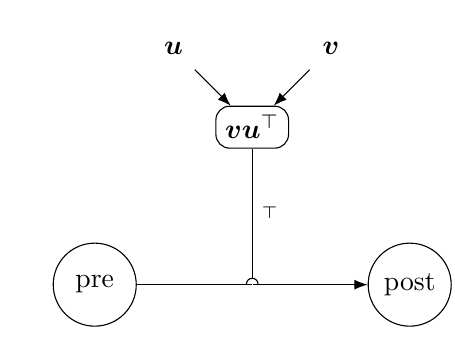
\begin{tikzpicture}[nef]
        \graph[no placement] {
            u/$\vc u$ [ext, at={(0, 0)}],
            v/$\vc v$ [ext, at={(2, 0)}],
            uv/$\vc v \vc u\Tr$ [net, at={(1, -1)}],
            u -> uv, v -> uv,
            pre [ens, at={(-1, -3)}, minimum size=30] -- mod/"" [minimum size=0, inner sep=0, at={(1, -3)}] -> post [ens, at={(3, -3)}, minimum size=30],
            uv -> [modulatory, "$\mdec\Tr$" right] mod,
        };
    \end{tikzpicture}
    \caption{Explicit neural calculation of the AML weight change.}\label{fig:aml-explicit}
\end{figure}

It might be surprising that the change in the connection weights between the pre- and post-ensemble does not depend on their own activity, but is controlled externally.
While this is different from many other common learning rules, there is evidence of such heterosynaptic learning in the brain and specifically the hippocampus \parencite{huilme2014,rebola2017,uchida2012}.
Furthermore, this learning rule requires some preexisting structure and connection weights to calculate the signal for the weight modulation.
But as most NEF models do not give a developmental account of how such structures come about, I put this question aside and leave it at something that has to be answered in the future and concerns any type of NEF model, not just this learning rule.
However, there is one more aspect that can be criticized as being biologically implausible: the connections from the outer product calculation depend on the decoders of the pre-population.
It is not clear how the pre-population could transmit this information to this other place.

A similar problem of biological plausibility occurs in classical neural networks and deep learning with back propagation, where the weights for the transmission of the error signal need to be symmetric to the forward weights.
Recently, this concern of biological plausibility in deep learning has been slightly alleviated by the discovery that the weight symmetry is not strictly required.
It is possible for the network to adjust its forward weights to account for existing, non-symmetric backward weights, a process known as feedback alignment \parencite{lillicrap2016}.
Unfortunately, it is not clear whether this can be applied to the situation here.


\section{Explicit calculation of weight change without weight symmetry}
By reformulating $\vc v(t) \vc u(t)\!\Tr \mdec$ as $\vc v(t)[\mdec\Tr \vc u(t)]\Tr$ it is possible to implement the learning rule without the need for a connection to be based on decoders of a neural ensemble it is not related to.
Again there is a set of neural ensembles calculating an outer product (see \cref{fig:aml-explicit-no-sym}).
\begin{figure}
    \centering
    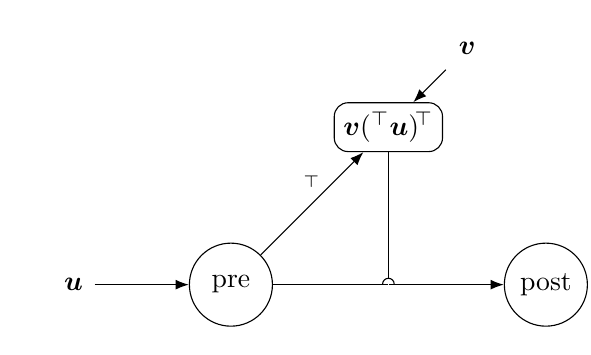
\begin{tikzpicture}[nef]
        \graph[no placement] {
            v/$\vc v$ [ext, at={(2, 0)}],
            uv/$\vc v (\mdec\Tr \vc u)\!\Tr$ [net, at={(1, -1)}],
            v -> uv,
            pre [ens, at={(-1, -3)}, minimum size=30] -- mod/"" [minimum size=0, inner sep=0, at={(1, -3)}] -> post [ens, at={(3, -3)}, minimum size=30],
            pre -> ["$\mdec\Tr$"] uv,
            uv -> [modulatory] mod,
            u/$\vc u$ [ext, at={(-3, -3)}] -> pre,
        };
    \end{tikzpicture}
    \caption{Explicit neural calculation of the AML weight change avoiding weight sharing.}\label{fig:aml-explicit-no-sym}
\end{figure}
But in contrast to the previous approach, if the pre-ensemble is also used as the cue input $\vc u(t)$, the transform $\mdec\Tr$ applied to $\vc u(t)$ is based on that ensemble's decoders decoding $\vc u(t)$.
The transform could even be rolled into the decoder matrix
\begin{equation}
    \mdec_{*} = \mdec\Tr \mdec \text{.}
\end{equation}
As we generally assume, in the context of the NEF, that there is some mechanism in place to establish the decoders to compute arbitrary given functions, this might already be considered a satisfactory answer to the biological plausibility.

However, it is not possible to state the function to obtain the decoders $\mdec_*$ because the function itself depends on the encoding by the neurons.
Moreover, $\mdec_*$ is a symmetric matrix, which is a constraint not respected by the normal decoder optimization process.
But in the context of the NEF, it can be assumed that the neural network can decode the identity function, i.e., there is a connection with decoders $\mdec$.
This can be used to learn a connection with decoders $\mdec_*$.

Given the vector of neural activities $\vc \act$ at time $t$, we have $\vc x = \mdec \vc \act$ and can state
\begin{equation}
    \vc x\Tr \vc x = \vc \act\Tr \mdec\Tr \mdec \vc\act \overset{!}{=} \vc\act\Tr\mdec_*\vc\act \text{.}
\end{equation}
This gives us an error expression as
\begin{equation}
    \err^2(\vc\act) = \left\lvert\vc x\Tr \vc x - \vc\act\Tr \mdec_* \vc\act\right\rvert^2 \overset{!}{=} 0
\end{equation}
with the gradient defined as
\begin{equation}
    \pd{\err^2(\vc\act)}{\mdec_*} = 2 \del{\vc\act\Tr \mdec_* \vc\act - \vc x\Tr \vc x} \del{\vc\act \vc\act\Tr} \text{.}
\end{equation}
The gradient can be used for a weight update rule
\begin{equation}
    \od{\mdec_*}{t} = -\eta_* \pd{\err^2(\vc\act)}{\mdec_*}
\end{equation}
in a (spiking) neural network to perform stochastic gradient descent.

To demonstrate that this learning rule allows the learning of the desired symmetric matrix, it was applied to a connection where the pre-synaptic ensemble was fed with a randomly varying vector signal.
The vector was generated from bandwidth limited Gaussian white noise (upper limit \SI{40}{\hertz}) for each component, normalized, and then multiplied by a bandwidth limited white noise scalar.
The learning rate was set to $\eta_* = \SI{1e-13}{\second^{-1}}$.
We can see that the Frobenius norm of the difference between the learned matrix $\mdec_*$ and the desired matrix $\mdec\Tr\mdec$ continuously decreases (\cref{fig:aml:grad-err}).
The decoded output for some dimensions quickly aligns with the target output (\cref{fig:aml:grad-decode}), but that does not happen for all dimensions.
This might be due to the random input not sufficiently covering the representational space.
\begin{figure}
    \centering
    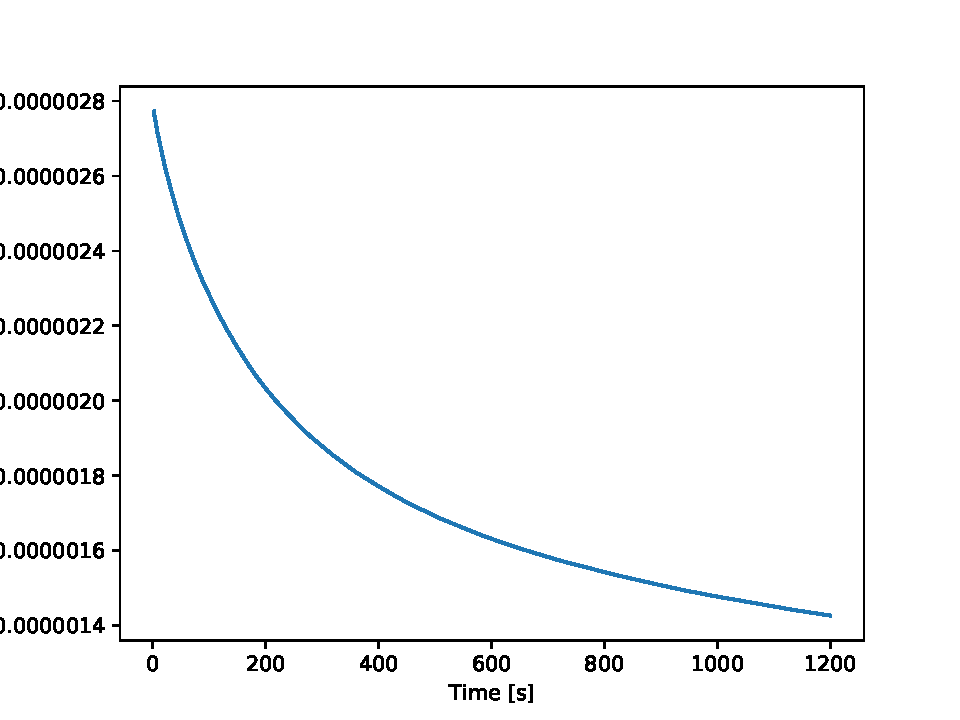
\includegraphics{figures/aml-grad-err}
    \caption{Error $\lVert \mdec\Tr\mdec - \mdec_*\rVert$.}\label{fig:aml:grad-err}
\end{figure}
\begin{figure}
    \centering
    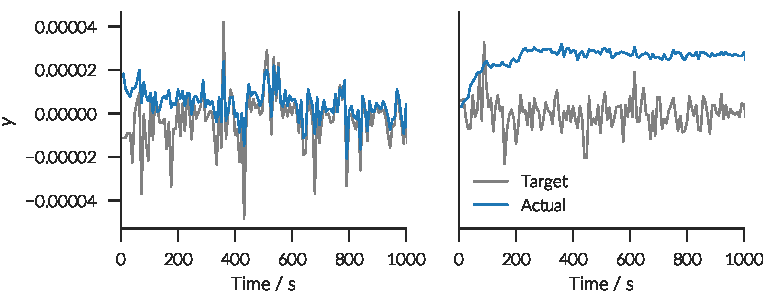
\includegraphics{figures/aml-decode}
    \caption[Example of two outputs decoded with the symmetric weights being learned.]{Example of two outputs decoded with the symmetric weights being learned. The output dimensions on the left quickly aligns with the target, while this does not happen (within the shown time frame) for the output dimension on the right.}\label{fig:aml:grad-decode}
\end{figure}

Again, the pure derivation of a learning rule does not ensure its biological plausibility.
Thus, let us consider the individual terms in the gradient.
The term $\vc\act\Tr \mdec_* \vc\act$ is using the current decoders to decode the ensemble's activity in no way different than usually done in the NEF where the existence of these standard decoders is generally assumed.
The decoded value is then correlated with the ensemble's activity.
The plausibility of this is somewhat unclear to the direct interaction of decoded values and neural activities, but to my knowledge there is no data excluding this possibility.
In particular, the decoded value and activities could be projected to another neural ensembles (see \cref{fig:aml-grad-desc}) that calculates the inner product.
The same, a projection to neural ensemble calculating the inner product, could happen with the decoded value $\vc x$.
Alternatively, $\vc x\Tr \vc x$ could directly be decoded (as a square of the individual components all projecting into the same dimension).
\Cref{fig:aml:neural-grad-err} shows the time course of the error when learning $\mdec_*$ with such a neural gradient computation.
The observed decrease demonstrates the basic viability of this approach, but the learning is slower and flattens out earlier due to the spiking noise.
\begin{figure}
    \centering
    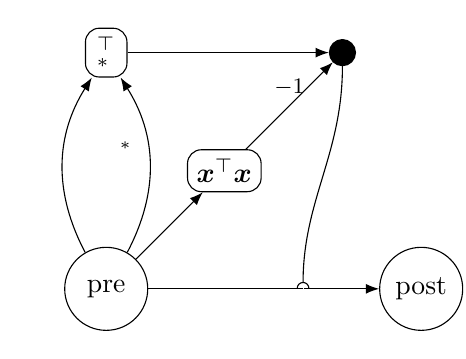
\begin{tikzpicture}[nef]
        \graph[no placement] {
            pre [ens, at={(0, 0)}, minimum size=30] -- mod/"" [inner sep=0, minimum size=0, at={(2.5, 0)}] -> post [ens, at={(4, 0)}, minimum size=30],
            pre -> [bend left] act/"$\vc\act\Tr \mdec_* \vc\act$" [net, at={(0, 3)}],
            pre -> [bend right, "$\mdec_*$" xshift=-3mm] act,
            pre -> targetact/"$\vc x\Tr \vc x$" [net, at={(1.5, 1.5)}],
            act -> combine/"" [pnode, at={(3, 3)}],
            targetact -> ["$-1$"] combine,
            combine -> [modulatory, out=270, in=90] mod,
        };
    \end{tikzpicture}
    \caption{Neural computation of the error signal necessary for learning symmetric decoders with gradient descent.}\label{fig:aml-grad-desc}
\end{figure}
\begin{figure}
    \centering
    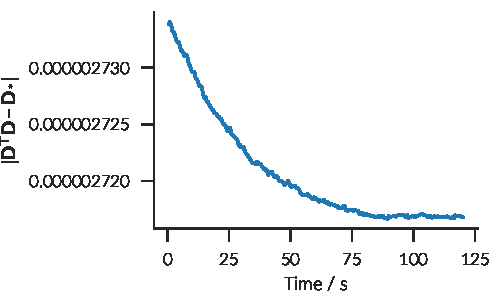
\includegraphics{figures/aml-neural-grad-err}
    \caption{Error $\lVert \mdec\Tr\mdec - \mdec_*\rVert$ with neural gradient calculation.}\label{fig:aml:neural-grad-err}
\end{figure}


The whole term $\vc\act\Tr \mdec_* \vc\act - \vc x\Tr \vc x$ is a scalar that influences all synapses.
This could be realized by a broadly acting neuro-modulator or by extensive connectivity of the neural ensembles calculating this error term.
Neither option is implausible.
This gradient term seems to play a role in weight normalization as it acts equally on all weights and the magnitude depends on the magnitude of the values of $\mdec_*$.
Also, without it all weight changes would always be negative.
Note that in many learning rules, normalization factors are often criticized as implausible for requiring knowledge of the whole weight matrix at the level of a single synapse.
This critique does not apply to this learning rule.
The decoding matrix is only used to decode from the activities which require only local knowledge of the weights.

Finally, the term $\vc\act \vc\act\Tr$ correlates neuron activities and appears somewhat Hebbian-like.
Hebbian learning is one of the best studied ways that biological systems learn.
In this form of learning pre- and post-synaptic neurons become connected when they fire in short succession.
In contrast to this usual account, here two pre-synaptic neurons connect to the same post-synaptic neuron if they fire together.
Again, the biological plausibility of this is somewhat uncertain, but cannot be outright rejected.


\section{Implicit error calculation}
The previous two implementations of the AML use minimal assumptions about the computational power of synapses.
All that is needed are additive weight changes proportional to some error signal.
However, it has been proposed that synapses might not simply transmit information, but also perform computations \parencites{abbott2004}[Ch.~5]{koch2004}.
In particular, \textcite{andreasstockel2018} showed that conductance-based synapses can be used in the NEF to compute nonlinear functions like multiplication.
That should allow us to roll the explicit outer product, required in the previous two approaches, into the synapses itself.
This requires considerably fewer neurons as no neural populations are required for each product.

In this thesis, I am using an implementation that corresponds to this implicit error calculation, but implements the required synaptic computation in pure math rather than implementing it with actual synaptic models.
This is mainly to reduce simulation times and is not meant as a statement that this is likely to correspond to the brain's implementation as there is not enough evidence to make such a strong claim.


\section{Normative interpretation}
While the AML cannot be outright rejected as biologically implausible, there are definitely some open questions concerning it.
Nevertheless, it should not be evaluated purely on this fact.
Many models in cognitive science, psychology, and computational neuroscience assume the encoding of associations in an outer product matrix \parencite[e.g.,][]{kajic2017,nowak2001,Brown2000}.
Ultimately, the validity of all those models depends on the possibility that the brain can learn such a matrix.
As such, the AML makes it explicit which operations have to be implemented to enable such learning.
If these turn out as either not being implemented in the brain or as not being implementable at all, it would follow that the brain has to use some other mechanism to represent associations.
Thus, the AML has merit as a normative theory, describing what the brain is ought to do, and directing research to open questions.

That being said, the AML does not make any assumption about the pre-synaptic neurons.
With such assumptions, some of the restrictions of the AML might be lessened.
For example, assuming orthogonal encoders, the decoder matrix $\mdec$ will be orthogonal too.
That in turn means that $\mdec_* = \mdec\Tr \mdec = \imat$ becomes the identity matrix which is independent of the exact decoders.
This simplifies connectivity and removes the need to learn the symmetric matrix $\mdec_*$ which alleviates some of the concerns of biological plausibility.

The dentate gyrus in the hippocampus is often assumed to perform pattern separation, which is a form of orthogonalization.
Hence, it might be possible that the hippocampus learns associations with a form of the AML where $\mdec_*$ ends up being the identity matrix and thus simplifies the learning rule itself.


\section{Properties of the AML}
So far the considerations about the AML were purely theoretical.
\Cref{fig:aml} demonstrates that an implementation of the AML can indeed learn associations in a spiking neural network.
Five different cue-target pairs were presented for one second each, before testing the recall with the same cues, but no target vectors.
The initially presented target vectors are almost perfectly recalled.
Note that no catastrophic forgetting occurred and each association was learned with a single presentation of the cue-target pair (one-shot learning).
Most other learning rules exhibit destructive interference between the items in this scenario.
As an example, \cref{fig:aml} also shows the same experiment using the Prescribed Error Sensitivity (PES) learning rule \parencite{bekolay2013}, which is commonly used in NEF models \parencite[e.g.,][]{komer2015,Rasmussen2017}.
Here all associations except for the last get destroyed.
It is still possible to learn associations with PES, but it requires the presentation of each item multiple times in interleaved fashion, i.e., one-shot learning cannot be done to learn associations in a reliable way.
\begin{figure}
    \centering
    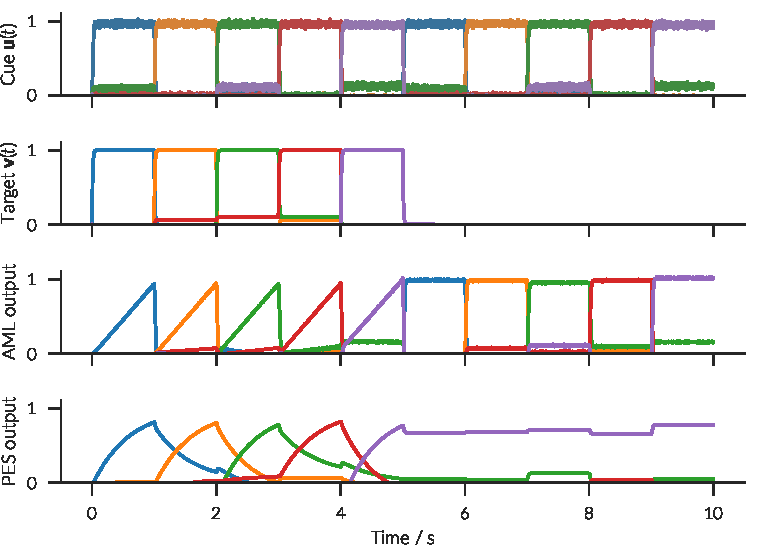
\includegraphics{figures/aml}
    \caption[Learning and recall testing of five cue-target pairs with the AML and PES.]{Learning and recall testing of five cue-target pairs with the AML and PES\@. Each colored trace is the dot product with one of the vectors used. The cue vectors $\vc u(t)$ and target vectors $\vc v(t)$ differ.}\label{fig:aml}
\end{figure}

This ability for one-shot learning with the AML is due to the $\mdec_*$ matrix, which accounts for the interference between neurons.
In fact, the AML and PES are the same except for that matrix.
The PES learning rule can be expressed as
\begin{equation}
    \od{\tilde{\mdec}}{t} = \eta \vc v(t) \vc\act_{\vc u}\Tr(t) \text{,}
\end{equation}
while the AML learning rule can be written as
\begin{equation}
    \od{\tilde{\mdec}}{t} = \eta \vc v(t) \vc u(t)\!\Tr \mdec = \eta \vc v(t) \vc\act_{\vc u}\Tr(t) \mdec\Tr \mdec
\end{equation}
which is the same, except for $\mdec_* = \mdec\Tr \mdec$.

The one-shot learning ability comes with some limitations, though.
The learning rule is restricted to learn transformations that can be expressed as outer product matrices, while learning rules like PES can learn arbitrary transformation matrices.
Moreover, the learning rule is essentially trying to learn a look-up table, mapping items to other items.
Thus, one should not expect the AML to generalize to unseen mappings.

This might be another reason, besides the stability-plasticity dilemma, why a two-stage memory system is needed.
The first stage would learn simple associations with the AML and only in the second step of consolidation with a different learning rule, commonalities get extracted for generalization.
This is consistent with data that shows that generalization improves with sleep.
For example, sleep improves transitive inference \parencite{stickgold2013-2} and gives insight into implicit rules \parencite{wagner2004}.
Experience replay in hippocampus might be responsible for the necessary interleaving of memory traces when using a learning rule that allows for more generalization, but exhibits destructive interference such as PES \parencite{mcclelland1995-1,kumaran2016}.
Overall, it is likely that AML only represents a first step in the association learning process and multiple learning rules are at play here.
That the brain uses no single general purpose learning rule, but combines different learning rules has been forcefully argued by \textcite{gallistel2009}.


\section{AML accounts for neural changes during association learning}\label{sec:aml-neural}
\Textcite{ison2015} reported that individual neurons in hippocampus (and parahippocampal cortex) change their firing rapidly to encode newly learned associations.
They recorded from the medial temporal lobe of \num{14} epilepsy patients that needed to undergo surgery.
They identified neurons that responded to specific visual stimuli of pictures of persons and landmarks and recorded the response to this \emph{preferred} (P) stimulus.
Then the participants learned associations between pairs of a person and a landmark.
Besides multiple tasks to assess the learning, the neuron responses to the different stimuli were recorded again after learning.

Pair-coding units could be identified that showed an elevated firing rate only to the preferred stimulus before learning (BL).
After learning (AL), those same units showed an elevated firing rate only to the preferred and associated non-preferred (NP) stimulus.
This can also be observed for associations learned with the AML\@.
\Cref{fig:aml-net} shows a NEF network that implements the learning of associations between persons and landmarks to reproduce the experiment by \textcite{ison2015}.
The connections weights from both pre-ensembles $\vc l$ and $\vc p$ are initialized with the identity transform.
To achieve firing rates closer to the recorded data, the maximum firing rates of the ensembles were sampled uniformly from \SIrange{10}{20}{\second^{-1}} (instead of \SIrange{200}{400}{\second^{-1}} used in the CUE model) and intercepts were sampled uniformly from \numrange{0.1}{1}.
The dimensionality of the ensembles and semantic pointers was set to \num{32}.
Furthermore, Gaussian white noise with a mean of \num{0.01} and standard deviation of \num{0.05}, low-pass filtered with a time-constant of \SI{0.1}{\second}, was injected into the neurons to account for neural background firing.
The recorded spikes were analyzed analogous to \textcite{ison2015}.
\begin{figure}
    \centering
    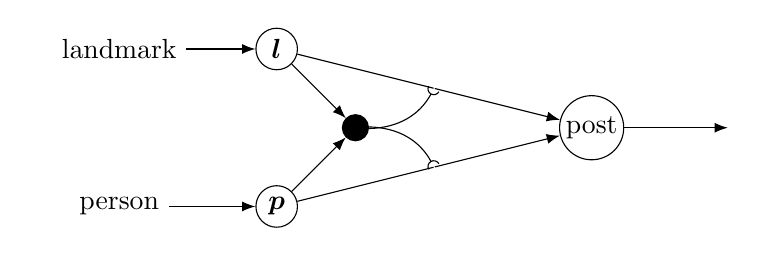
\begin{tikzpicture}[nef]
        \graph [no placement] {
            landmark [x=-2, y=0, ext] -> L/"$\vc l$" [x=0, y=0, ens] -- c1/"" [inner sep=0, minimum size=0, x=2, y=-0.5] -> post [x=4, y=-1, ens];
            person [x=-2, y=-2, ext] -> P/"$\vc p$" [x=0, y=-2, ens] -- c2/"" [inner sep=0, minimum size=0, x=2, y=-1.5] -> post;
            L -> err/"" [x=1, y=-1, pnode] -> [bend right, modulatory] c1;
            P -> err -> [bend left, modulatory] c2;
            post -> output/"" [x=6, y=-1, ext];
        };
    \end{tikzpicture}
    \caption[NEF network for associating two stimuli with the AML.]{NEF network for associating two stimuli (persons with landmarks here) with the AML.}\label{fig:aml-net}
\end{figure}

The main results obtained from the experimental and model data are shown in Figs.~\ref{fig:aml-spikes} and~\ref{fig:aml-population-response}.
\begin{figure}
    \centering
    \subcaptionbox{Experimental data}{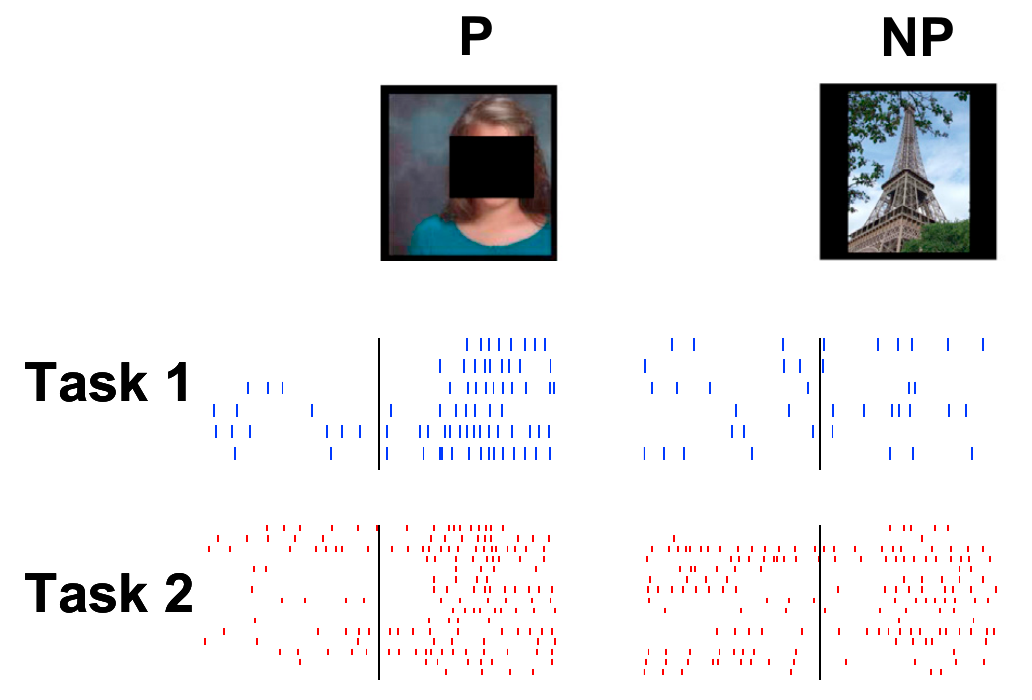
\includegraphics[width=9cm]{figures/ison2015-spikes}}

    \vspace*{0.34cm}
    \subcaptionbox{Model data}{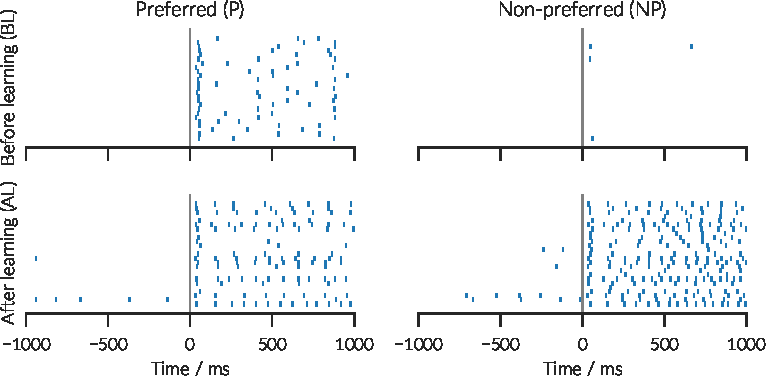
\includegraphics{figures/aml-spikes}}
    \caption[Change in spiking behaviour when learning associations.]{Change in spiking behaviour when learning associations. (a) Exemplary spikes recorded from human hippocampus for the preferred (P) and non-preferred (NP) stimulus. Task 1 (blue) is before, task 2 (red) after learning the P-NP association. The black line marks the stimulus onset. Figure adopted from \textcite{ison2015} under the Creative Commons Attribution 4.0 International license. (b) Spikes recorded from the NEF model learning the P-NP association with the AML\@.}\label{fig:aml-spikes}
\end{figure}
\begin{figure}
    \centering
    \subcaptionbox{Experimental data}{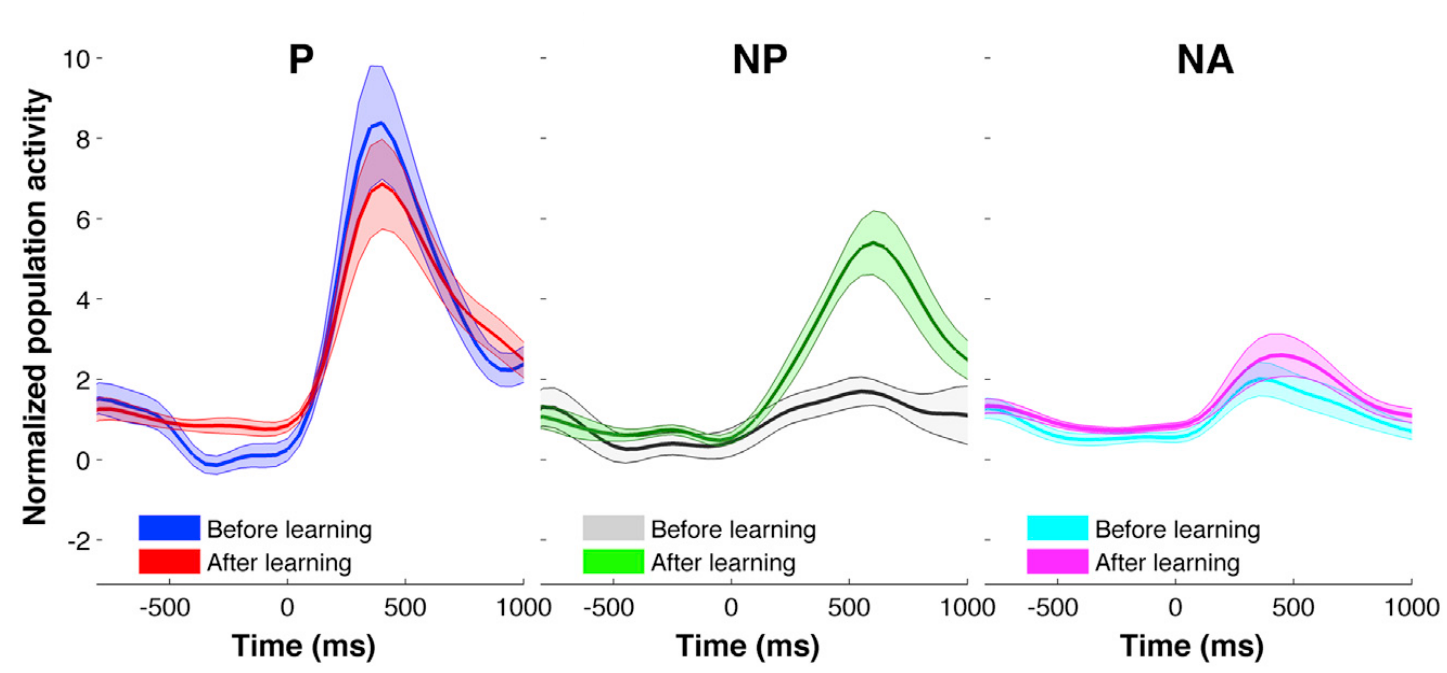
\includegraphics[width=12cm]{figures/ison2015-pop}}

    \vspace*{.75cm}
    \subcaptionbox{Model data}{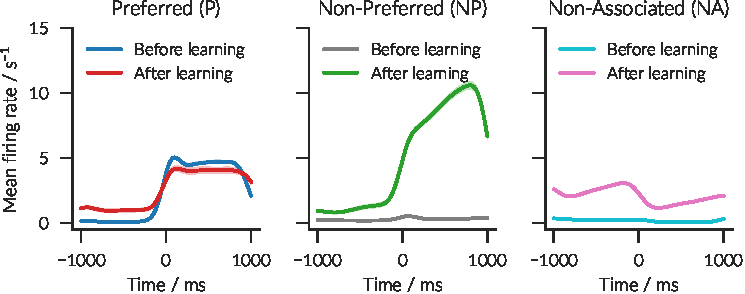
\includegraphics{figures/aml-population-response}}
    \caption[Population response for pair-coding units.]{Population response for pair-coding units to the preferred (P), non-preferred (NP), and non-associated (NA) stimuli before and after learning. Times are relative to stimulus onset. Shaded regions indicate the standard error of mean. (a) Normalized population activity from (a) experimental and (b) model data. Figure (a) adopted from \textcite{ison2015} under the Creative Commons Attribution 4.0 International license.}\label{fig:aml-population-response}
\end{figure}
Pairwise coding units, showing elevated firing in response to the preferred stimulus before learning and the non-preferred stimulus after learning without an increased response to any other stimuli, have been selected.
The normalized population activity in response to the preferred stimulus shows no or only a minimal change with learning in both the experimental and model data.
For the non-preferred stimulus the population activity increases slightly on stimulus onset which is more pronounced in the model data.
This might be explained by the model not including any visual processing that could delay and smooth out that response.
After learning, this population response is increased in both sets of data.
For non-associated stimuli the model shows a minimal decrease in the normalized population activity with learning, while the experimental data shows no significant change.
Overall, the model matches the main aspects of the experimental observations.
A better quantitative fit might be achievable with more careful parameter selection in the model.


\section{Weight normalization}
Note that the AML allows weights to grow without bound.
By introducing a factor of $1 - \vc v(t)\!\Tr \hat{\vc v}(t)$ this can be prevented where $\hat{\vc v}(t)$ is the retrieved, learned association.
But similar to other weight normalizations it introduces the need for each weight to have access to the global population activity and weights as $\hat{\vc v}(t) = \tilde{\mdec} \vc\act_{\vc u}(t)$.
Such global dependencies are often criticized for not being biologically plausible.
As such, I decided to take a slightly different approach with an equivalent effect.
Instead of including the dot product $\vc v(t)\!\Tr \hat{\vc v}(t)$ in the learning rule, it can be computed by another neural population and the thresholded result can be used to inhibit the population providing $\vc v$.
Once fully inhibited, $\vc\act_{\vc v}(t)$ will be all-zero and thus prevent further weight changes.
In the CUE model, the inhibition threshold is adjusted to follow $1 + \exp(-t)$ for learning the $\mtf$ matrix where $t$ is the time since the trial started.
This is intended to account for rehearsal effects that are not explicitly modelled and is analogous to the extended TCM model by \textcite{Sederberg2008}.

\chapter{Recalling items}
(WTA mechanisms)
\chapter{The complete model}
\chapter{Results}
\chapter{Discussion}
\chapter{Conclusion}

\chapter{Acknowledgements}
IK
%----------------------------------------------------------------------
% END MATERIAL
%----------------------------------------------------------------------

% B I B L I O G R A P H Y
% -----------------------

% The following statement selects the style to use for references.  It controls the sort order of the entries in the bibliography and also the formatting for the in-text labels.
%\bibliographystyle{plain}
% This specifies the location of the file containing the bibliographic information.  
% It assumes you're using BibTeX (if not, why not?).
\cleardoublepage % This is needed if the book class is used, to place the anchor in the correct page,
                 % because the bibliography will start on its own page.
                 % Use \clearpage instead if the document class uses the "oneside" argument
\phantomsection  % With hyperref package, enables hyperlinking from the table of contents to bibliography             
% The following statement causes the title "References" to be used for the bibliography section:
\renewcommand*{\bibname}{References}

% Add the References to the Table of Contents
\addcontentsline{toc}{chapter}{\textbf{References}}

% Tip 5: You can create multiple .bib files to organize your references.  Just 
% list them all in the \bibliogaphy command, separated by commas (no spaces).

% The following statement causes the specified references to be added to the bibliography% even if they were not 
% cited in the text. The asterisk is a wildcard that causes all entries in the bibliographic database to be included (optional).
\nocite{*}
\printbibliography

% The \appendix statement indicates the beginning of the appendices.
\appendix
% Add a title page before the appendices and a line in the Table of Contents
\chapter*{APPENDICES}
\addcontentsline{toc}{chapter}{APPENDICES}
%======================================================================
\chapter[PDF Plots From Matlab]{Matlab Code for Making a PDF Plot}
\label{AppendixA}
% Tip 4: Example of how to get a shorter chapter title for the Table of Contents 
%======================================================================

\end{document}
